\chapter{Thực nghiệm và kết quả}
\label{chap:experiment}

Trong phần này, chúng ta sẽ xem xét kết quả thực nghiệm thu được khi áp dụng ALNS cho VRPTW với hai tập dữ liệu của Solomon (1987) \cite{solomon1987algorithms} và Gehring, Hermann, Homberger (1999) \cite{gehring1999parallel}. Ở cả hai tập, các bộ dữ liệu được chia thành 3 loại C, R và RC. Với dữ liệu lớp C, các yêu cầu được phân thành các cụm rõ rệt, lớp R là hoàn toàn ngẫu nhiên và lớp RC là sự kết hợp của hai lớp trên. Tác giả chỉ xem xét các tập từ 100 yêu cầu trở lên (bỏ qua tập Solomon 25, 50 yêu cầu vì nhìn chung số lượng yêu cầu như vậy là quá nhỏ để nhận thấy sự khác biệt khi so sánh ALNS với các thuật toán khác).

\begin{figure}[H] % places figure environment here   
	\label{fig:perf_ct_c1}
	\begin{subfigure}{.3\textwidth}
		\centering
		
\includegraphics[width=1\linewidth]{figures/cls_c.png}
		\caption{Lớp C}
		\label{fig:cls_c}
	\end{subfigure}%
	\begin{subfigure}{.3\textwidth}
		\centering
		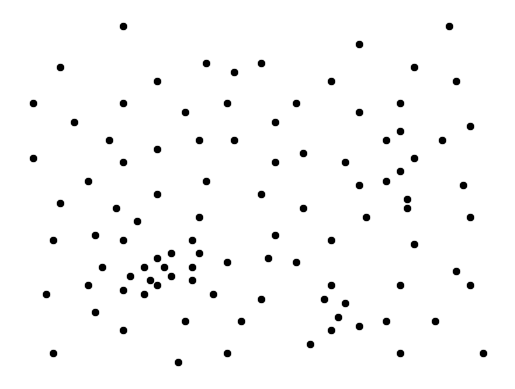
\includegraphics[width=1\linewidth]{figures/cls_r.png}
		\caption{Lớp R}
		\label{fig:cls_r}
	\end{subfigure}
	\begin{subfigure}{.3\textwidth}
		\centering
		
\includegraphics[width=1\linewidth]{figures/cls_rc.png}
		\caption{Lớp RC}
		\label{fig:cls_rc}
	\end{subfigure}
	\caption{Lớp các cấu hình}
\end{figure}

\begin{figure}[H] % places figure environment here   
	\label{fig:perf_ct_c2}
	\begin{subfigure}{.3\textwidth}
		\centering
		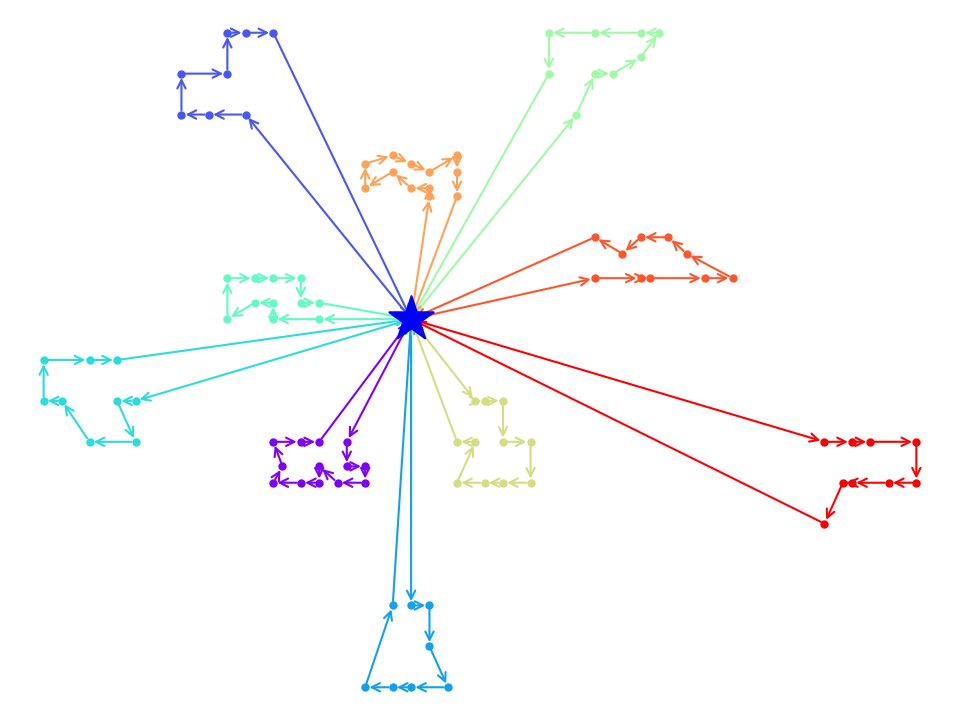
\includegraphics[width=1\linewidth]{figures/routes_c101.png}
		\caption{Lớp C}
		\label{fig:route_c}
	\end{subfigure}%
	\begin{subfigure}{.3\textwidth}
		\centering
		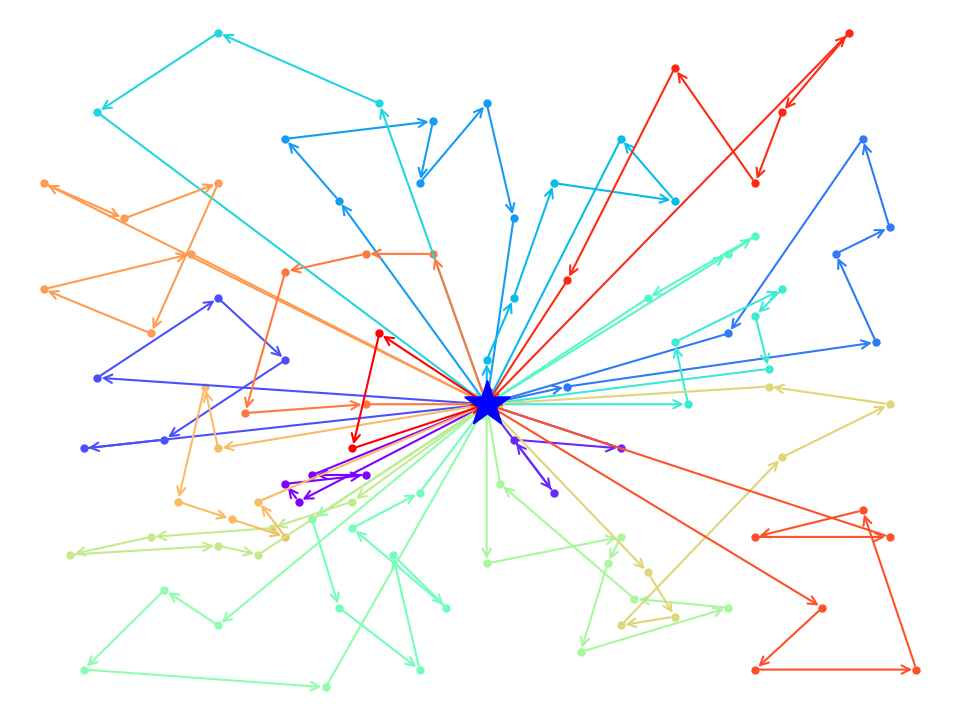
\includegraphics[width=1\linewidth]{figures/routes_r101.png}
		\caption{Lớp R}
		\label{fig:route_r}
	\end{subfigure}
	\begin{subfigure}{.3\textwidth}
		\centering
		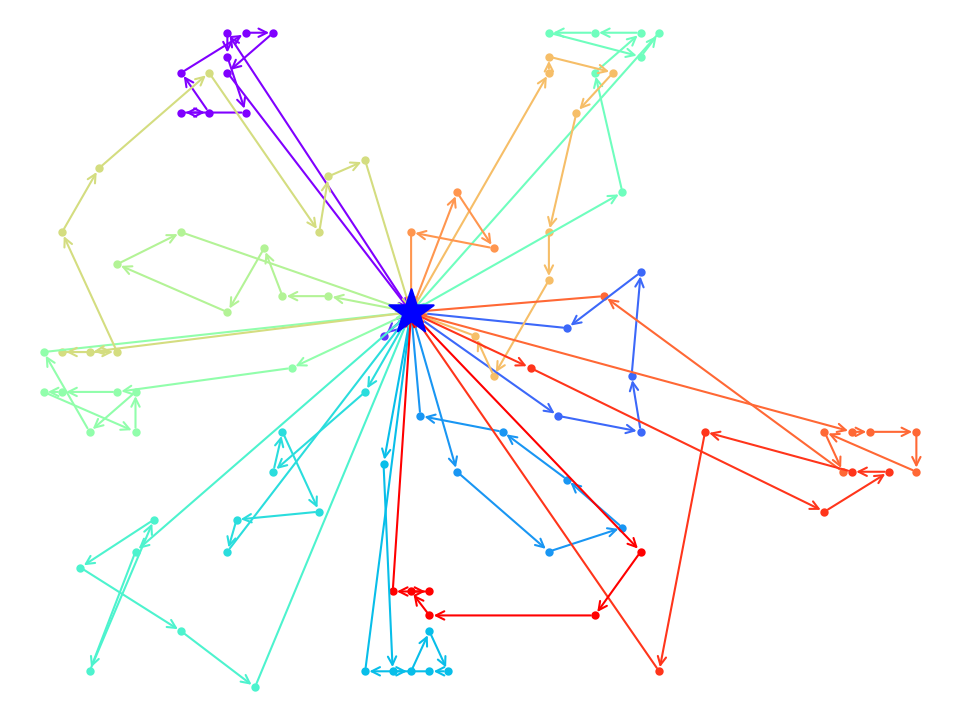
\includegraphics[width=1\linewidth]{figures/routes_rc101.png}
		\caption{Lớp RC}
		\label{fig:route_rc}
	\end{subfigure}
	\caption{Minh họa lời giải cho các lớp cấu hình}
\end{figure}

Thí nghiệm được chạy trên CPU Intel Xeon E5-2680 v4 @ 2.40GHz với Ubuntu 22.04.1 LTS. Mã nguồn được viết bằng ngôn ngữ C++ và được biên dịch bằng GCC 11.4.0 với các tùy chọn tối ưu hóa -O3. Chương trình được chạy với 8 luồng.

\section{Chất lượng nghiệm}

Trong phần này, tác giả đưa ra các số liệu thực nghiệm về giá trị hàm mục tiêu khi áp dụng ALNS giải VRPTW. Do thuật toán sử dụng rất nhiều tham số ngẫu nhiên nên chúng ta không tiến hành chạy một lần mà chạy nhiều lần để thu được kết quả tốt nhất cũng như kết quả trung bình và đánh giá độ ổn định của thuật toán. Độ ổn định được đánh giá bằng độ lệch chuẩn của các kết quả đo giá trị hàm mục tiêu. Thực tế số lần chạy không quá lớn do thời gian chạy mỗi cấu hình là khá lâu nhưng tác giả vẫn cố gắng đưa vào độ đo độ lệch chuẩn để phần nào đánh giá được độ ổn định của thuật toán. Về mặt thống kê, điều này chưa hẳn là đúng đắn tuy nhiên ta vẫn thấy được một phần sự ổn định của ALNS qua các kết quả đo được. Số xe được sử dụng cũng được tác giả chỉ ra. Ta biết rằng số xe sử dụng ảnh hưởng rất nhiều đến hàm mục tiêu. Về cơ bản, khi có quá nhiều xe được sử dụng thì chất lượng nghiệm là tệ. Lâu dài, khi hàm mục tiêu "gần" hơn với giá trị tối ưu thì số xe cũng ổn định ở một mức nào đó và nhìn chung là giảm so với nghiệm ban đầu (được khởi tạo). Các kết quả sau đó được so sánh với nghiệm tốt nhất đã biết được lấy từ trang CVRPLIB (\href{http://vrp.galgos.inf.puc-rio.br/index.php/en/}{http://vrp.galgos.inf.puc-rio.br/index.php/en/}). Sintef (\href{https://www.sintef.no/}{https://www.sintef.no/}) cũng là một nguồn được sử dụng khá rộng rãi trong các bài báo khoa học nhưng nghiệm được báo cáo có chất lượng không tốt bằng CVRPLIB. 

\subsection{Số lượng yêu cầu liệu nhỏ}
\label{sec:exp_small}

Trước tiên, chúng ta bắt đầu với tập dữ liệu Solomon (1987) được đưa ra bởi Solomon (1987) \cite{solomon1987algorithms}. Solomon (1987) là một tập dữ liệu nổi tiếng được sử dụng để đánh giá chất lượng trong hầu hết các nghiên cứu về VRP. Các cấu hình và nghiệm được định dạng tiêu chuẩn bao gồm tên cấu hình, số xe tối đa dược sử dụng, tải trọng mỗi xe, ID của yêu cầu, tọa độ của các yêu cầu, nhu cầu (về tải) của mỗi yêu cầu, khung thời gian và thời gian phục vụ tại mỗi yêu cầu. Thông tin về kho được cho bởi ID 0. Với các cấu hình theo tiêu chuẩn định dạng Solomon (kể cả các cấu hình khác ngoài Solomon (1987)), tốc độ của xe được hiểu là 1 đơn vị; nói cách khác, thời gian di chuyển giữa các yêu cầu bằng với khoảng các giữa chúng. 

Tập dữ liệu được chia thành 3 lớp C, R và RC. Solomon sinh hai tập loại 1 và loại 2. Quy tắc đặt tên \code{\{class\}\{type\}\{num\}} với \code{class} là lớp C, R hoặc RC, \code{type} là loại 1 hoặc 2, \code{num} là số thứ tự của cấu hình. Mỗi lớp có từ $8$ đến $12$ cấu hình. Các cấu hình cũng được chia thành ba nhóm với $25$, $50$ và $100$ yêu cầu. Trong luận văn này, tác giả chỉ đưa ra các kết quả cho các tập $100$ yêu cầu do các cấu hình $25$ hay $50$ yêu cầu là khá nhỏ và ta không thấy rõ sự khác biệt do hầu hết các thuật toán đều cho kết quả rất tốt.

\begin{table}[caption={Kết quả đo với tập Solomon C}, label=exp:solomonC]
  \begin{adjustbox}{width=1\textwidth}
  \small
  \begin{tabularx}{\textwidth}{|XXXXXX|XXXXXX|}
  \hline
  ins & cost & nv & bkcost & bknv & gap & ins & cost & nv & bkcost & bknv & gap \\ \hline
  c101 & 828.94 & 10 & 827.30 & 10 & 0.20 & c201 & 591.56 & 3 & 589.10 & 3 & 0.42 \\ \hline
  c102 & 828.94 & 10 & 827.30 & 10 & 0.20 & c202 & 591.56 & 3 & 589.10 & 3 & 0.42 \\ \hline
  c103 & 828.06 & 10 & 826.30 & 10 & 0.21 & c203 & 591.17 & 3 & 588.70 & 3 & 0.42 \\ \hline
  c104 & 824.78 & 10 & 822.90 & 10 & 0.23 & c204 & 590.60 & 3 & 588.10 & 3 & 0.42 \\ \hline
  c105 & 828.94 & 10 & 827.30 & 10 & 0.20 & c205 & 588.88 & 3 & 586.40 & 3 & 0.42 \\ \hline
  c106 & 828.94 & 10 & 827.30 & 10 & 0.20 & c206 & 588.49 & 3 & 586.00 & 3 & 0.43 \\ \hline
  c107 & 828.94 & 10 & 827.30 & 10 & 0.20 & c207 & 588.29 & 3 & 585.80 & 3 & 0.42 \\ \hline
  c108 & 828.94 & 10 & 827.30 & 10 & 0.20 & c208 & 588.32 & 3 & 585.80 & 3 & 0.43 \\ \hline
  c109 & 828.94 & 10 & 827.30 & 10 & 0.20 &  &  &  &  &  &  \\ \hline
  avg & & & & & 0.20 &  &  &  &  & & 0.42 \\ \hline
  \end{tabularx}
  \end{adjustbox}
  \end{table}

  \textit{ Trong đó
    \begin{itemize}
      \item[-] ins: cấu hình
      \item[-] cost: chi phí thu được với ALNS
      \item[-] nv: số xe được sử dụng
      \item[-] bkcost: chi phí tốt nhất đã biết
      \item[-] bknv: số xe tốt nhất đã biết
      \item[-] gap (\%): khoảng cách so với nghiệm tốt nhất đã biết
      \item[-] avg: trung bình cộng các giá trị theo cột tương ứng
    \end{itemize}
  }

  Với các cấu hình loại C, ALNS cho nghiệm cách nghiệm tốt nhất đã biết trung bình $0.20\%$ và $0.42\%$ cho C1 và C2. Trong thực tế, đối với các doanh nghiệp giao vận nhỏ, hoặc một nhóm người giao hàng thì số lượng yêu cầu như vậy là bình thường. Các nhóm giao hàng nhỏ thường nhận các yêu cầu được phân cụm một cách tương đối (theo khu vực địa lý) như vậy. 

  Thí nghiệm được thiết lập có thời gian timeout một phút, chạy năm lần và lấy kết quả tốt nhất. Tập C1 và C2 tương đối nhỏ và đã phân cụm nên trong thực tế thuật toán chạy rất nhanh để ra được nghiệm tốt và không có sự khác biệt giữa các lần chạy, trên CPU được thí nghiệm, ALNS mất dưới 1 giây để tìm ra nghiệm kém hơn nghiệm tốt nhất đã biết dưới $1\%$.

  \begin{table}[caption={Kết quả đo với tập Solomon R1}, label=exp:solomonR1]
    % \begin{adjustbox}{width=1\textwidth}
    \small
    \centering
    \begin{tabular}{lrrrll}
    \hline
    instance & alns best & nv & bkcost & bknv & gap (\%) \\ \hline
    r101 & 1,642.88 & 20 & 1,637.70 & 20 & 0.32 \\ \hline
    r102 & 1,472.81 & 18 & 1,466.60 & 18 & 0.42 \\ \hline
    r103 & 1,213.62 & 15 & 1,208.70 & 14 & 0.41 \\ \hline
    r104 & 976.61 & 11 & 971.50 & 11 & 0.53 \\ \hline
    r105 & 1,360.78 & 15 & 1,355.30 & 15 & 0.40 \\ \hline
    r106 & 1,239.37 & 13 & 1,234.60 & 13 & 0.39 \\ \hline
    r107 & 1,073.60 & 12 & 1,064.60 & 11 & 0.85 \\ \hline
    r108 & 944.44 & 10 & 932.10 & 10 & 1.32 \\ \hline
    r109 & 1,152.38 & 13 & 1,146.90 & 13 & 0.48 \\ \hline
    r110 & 1,078.59 & 12 & 1,068.00 & 12 & 0.99 \\ \hline
    r111 & 1,053.50 & 12 & 1,048.70 & 12 & 0.46 \\ \hline
    r112 & \text{955.68} & 10 & \text{948.60} & \text{10} & \text{0.75} \\ \hline
    avg &  &  &  &  & 0.61 \\ \hline
    \end{tabular}
    % \end{adjustbox}
  \end{table}

  Tập R1 và R2 có các yêu cầu được tạo hoàn toàn ngẫu nhiên thế nên cũng có nhiều nghiệm chấp nhận được và thuật toán cũng khó bị bẫy ở một nghiệm tối ưu địa phương. Tuy nhiên, thuật toán cũng mất nhiều thời gian để tìm nghiệm tối ưu hơn do có nhiều nghiệm thỏa mãn các ràng buộc. Riêng với tập R2, ALNS đã tìm ra nghiệm với số xe ít hơn nghiệm tốt nhất đã biết mà tổng khoảng cách chỉ chênh lệch nhỏ. Lớp R có thể được sử dụng để mô phỏng các yêu cầu ở những vùng thưa dân cư như nông thôn chẳng hạn. Các yêu cầu thưa thớt hơn ở thành phố và khoảng cách giữa các yêu cầu cũng không gần nhau (các yêu cầu không tập trung thành các cụm rõ rệt). Việc đặt số lượng lớn các bưu cục ở vùng nông thôn là không khả thi về mặt chi phí vận hành cho các doanh nghiệp. Như vậy, sử dụng một thuật toán tối ưu nào đó là tiết kiệm chi phí (quãng đường) rất nhiều so với việc giao hàng một cách ngẫu nhiên hay theo quy tắc "tham lam". 

  \begin{table}[caption={Kết quả đo với tập Solomon R2}, label=exp:solomonR2, placement=h]
    % \begin{adjustbox}{width=1\textwidth}
    \small
    \centering
    \begin{tabular}{lrrrll}
    \hline
    instance & alns best & nv & bkcost & bknv & gap (\%) \\ \hline
    r201 & 1,152.96 & \textbf{7} & 1,143.20 & 8 & 0.32 \\ \hline
    r202 & 1,035.32 & \textbf{7} & 1,029.60 & 8 & 0.42 \\ \hline
    r203 & 880.90 & 6 & 870.80 & 6 & 0.41 \\ \hline
    r204 & 743.91 & \textbf{4} & 731.30 & 5 & 0.53 \\ \hline
    r205 & 958.81 & 5 & 949.80 & 5 & 0.40 \\ \hline
    r206 & 883.92 & 5 & 875.90 & 5 & 0.39 \\ \hline
    r207 & 806.31 & 5 & 794.00 & 4 & 0.85 \\ \hline
    r208 & 948.57 & 4 & 701.00 & 4 & 1.77 \\ \hline
    r209 & 717.53 & 5 & 854.80 & 5 & 0.48 \\ \hline
    r210 & 909.32 & \textbf{5} & 900.50 & 6 & 0.99 \\ \hline
    r211 & 1,053.50 & 5 & 746.70 & 4 & 0.46 \\ \hline
    avg &  &  &  &  & 1.38 \\ \hline
    \end{tabular}
    % \end{adjustbox}
  \end{table}

  \begin{table}[caption={Kết quả đo với tập Solomon RC1}, label=exp:solomonRC1, placement=h]
    % \begin{adjustbox}{width=1\textwidth}
    \small
    \centering
    \begin{tabular}{rrrrrr}
    \hline
    instance & alns best & nv & bkcost & bknv & gap (\%) \\ \hline
    rc101 & 1,623.58 & 16 & 1,619.80 & 15 & 0.23 \\ \hline
    rc102 & 1,461.23 & 14 & 1,457.40 & 14 & 0.26 \\ \hline
    rc103 & 1,266.62 & 11 & 1,258.00 & 11 & 0.69 \\ \hline
    rc104 & 1,136.91 & 10 & 1,132.30 & 10 & 0.41 \\ \hline
    rc105 & 1,518.58 & 16 & 1,513.70 & 15 & 0.32 \\ \hline
    rc106 & 1,376.99 & 13 & 1,372.70 & 12 & 0.31 \\ \hline
    rc107 & 1,211.11 & 12 & 1,207.80 & 12 & 0.27 \\ \hline
    rc108 & 1,118.13 & 11 & 1,114.20 & 11 & 0.35 \\ \hline
    avg &  &  &  &  & 0.36 \\ \hline
    \end{tabular}
    % \end{adjustbox}
  \end{table}

  \begin{table}[caption={Kết quả đo với tập Solomon RC2}, label=exp:solomonRC2, placement=h]
    % \begin{adjustbox}{width=1\textwidth}
    \small
    \centering
    \begin{tabular}{rrrrrr}
    \hline
    instance & alns best & nv & bkcost & bknv & gap (\%) \\ \hline
    rc201 & 1,274.61 & \textbf{8} & 1,261.80 & 9 & 1.02 \\ \hline
    rc202 & 1,099.54 & \textbf{6} & 1,092.30 & 8 & 0.66 \\ \hline
    rc203 & 931.16 & 5 & 923.70 & 5 & 0.81 \\ \hline
    rc204 & 788.66 & 4 & 783.50 & 4 & 0.66 \\ \hline
    rc205 & 1,157.66 & 7 & 1,154.00 & 7 & 0.32 \\ \hline
    rc206 & 1,060.50 & \textbf{6} & 1,051.10 & 7 & 0.89 \\ \hline
    rc207 & 966.08 & 6 & 962.90 & 6 & 0.33 \\ \hline
    rc208 & 785.73 & 4 & 776.10 & 4 & 1.24 \\ \hline
    avg &  &  &  &  & 0.74 \\ \hline
    \end{tabular}
    % \end{adjustbox}
  \end{table}

  Tương tự như lớp R, ALNS vẫn thể hiện rất tốt cho cấu hình lớp RC khi cho khoảng cách trung bình so với nghiệm tốt nhất đã biết là $0.36\%$ và $0.74\%$ cho RC1 và RC2. Với một số cầu hình \code{rc201}, \code{rc202} và \code{rc206}, ALNS cũng tìm được nghiệm với số xe ít hơn so với nghiệm tốt nhất đã biết. Việc tiết kiệm được số xe về tổng thể là rất có ý nghĩa trong thực tế  bởi chi phí thuê hay mua xe, trả lương cho tài xế và vận hành... là lớn hơn nhiều so với khi tiết kiệm được một vài phần trăm về quãng đường. Tuy nhiên, với một số cấu hình \code{rc1}, ALNS sử dụng nhiều xe hơn.

  Nhìn chung, với tập dữ liệu dưới $100$ yêu cầu, ALNS luôn cho kết quả tốt với số xe cần sử dụng ít. Trong quá trình thực nhiệm, tác giả cũng nhận thấy các kết quả chênh lệch nhau rất ít giữa các lần chạy (dưới $1\%$). Như vậy, ta có thể đưa ra một nhận xét sớm rằng ALNS đáp ứng tốt cho các cấu hình VRPTW với số lượng yêu cầu nhỏ (dưới $100$ yêu cầu). Điều này gợi ý sử dụng ALNS cho các bài toán thực tế của doanh nghiệp nhỏ hoặc ít nhất là cho các bưu cục (ở các khu vực khác nhau) của các doanh nghiệp lớn.
  
  % Ngoài ra, ALNS chứng tỏ được sự ổn định và có hiệu năng đủ tốt (sẽ được trình bày ở phần \ref{sec:performance}) ngay cả với các cấu hình với số lượng yêu cầu rất lớn. Điều này gợi ý sử dụng ALNS cho các bài toán thực tế của doanh nghiệp nhỏ hoặc ít nhất là cho các bưu cục (ở các khu vực khác nhau) của các doanh nghiệp lớn. Mặc dù đã được đề xuất từ khá lâu (1987), nhưng tập Solomon (1987) vẫn chứng tỏ được giá trị của nó đối với các bài thí nghiệm hiện đại và có tính ứng dụng cao trong thực tế. Tác giả không đưa vào các kết quả trung bình của các lần chạy thuật toán và độ lệch chuẩn do tập dữ liệu khá nhỏ. Các độ đo này sẽ được trình bày trong phần tiếp theo với số lượng yêu cầu từ trung bình ($200$, $400$), lớn ($400$, $600$) và rất lớn ($800$, $1000$).

  \subsection{Số lượng yêu cầu lớn và rất lớn}
  \label{sec:exp_large}
  
  Trong phần này, tác giả tiến hành thực nghiệm ALNS với tập dữ liệu lớn hơn với số lượng yêu cầu từ $200$ lên tới $1000$. Về con số $1000$ so với $100$ không làm chúng ta cảm thấy sự khác biệt, nhưng lưu ý rằng, độ phức tạp của bài toán là giai thừa, $O(1000!)$ là một con số lớn khủng khiếp! Tập dữ liệu được sử dụng được sinh trong Gehring, Hermann, Homberger (1999) \cite{gehring1999parallel} (sau đây tác giả gọi là tập HG cho ngắn gọn). Các cấu hình được ghi theo tiêu chuẩn Solomon đã được trình bày trong phần \ref{sec:exp_small}. Quy tắc đặt tên được quy ước như sau \code{\{class\}\{type\}\_\{size\}\_\{num\}} với \code{class} là lớp cấu hình C, R hay RC; \code{type} là loại $1$ hoặc $2$ (tương tự như tập Solomon (1987), HG cũng được sinh 2 bộ dữ liệu); \code{size} là kích thước cấu hình (ví dụ $2$ là $200$ yêu cầu, $8$ là $800$ yêu cầu); \code{num} là số thứ tự của cấu hình.

  Với số lượng yêu cầu là 200, ALNS vẫn tỏ ra hiệu quả với thời gian timeout một phút. ALNS cho chênh lệch trung bình $0.23\%$, $1.60\%$ và $1.73\%$ lần lượt cho các lớp C, R, RC so với nghiệm tốt nhất đã biết. Ngoài ra, ALNS tỏ ra ổn định khi độ lệch chuẩn giữa các lần chạy là rất nhỏ khi so sánh với giá trị hàm mục tiêu. Số xe sử dụng cũng không có sự khác biệt so với nghiệm tốt nhất đã biết.

  Đối với tập 400 yêu cầu, ALNS cho kết quả không tốt như với các tập có số lượng yêu cầu nhỏ với thời gian timeout một phút. Độ chênh lệch trung bình lần lượt là $1.99\%$, $4.35\%$ và $5.78\%$ cho lớp C, R và RC khi so sánh với nghiệm tốt nhất đã biết. Ta có thể thấy rằng, đối với lớp khó như RC, ALNS không còn duy trì được hiệu quả như khi giải bài toán lớp C và R. Tuy nhiên, ALNS vẫn ổn định khi độ lệch chuẩn giữa các lần đo vẫn rất nhỏ so với giá trị hàm mục tiêu. 

  Dưới đây là các kết quả đo cho các cấu hình 200, 400, 600, 800 và 1000 yêu cầu cho 3 lớp C, R và RC. 

  \textit{Trong đó
  \begin{itemize}
    \item[-] ins: tên cấu hình
    \item[-] alns best: giá trị hàm mục tiêu tốt nhất đạt được bởi ALNS
    \item[-] alns avg: giá trị hàm mục tiêu trung bình (với 5 lần đo) đạt được bởi ALNS
    \item[-] alns std: độ lệch chuẩn của giá trị hàm mục tiêu (với 5 lần đo) đạt được bởi ALNS
    \item[-] nv: số xe được sử dụng bởi ALNS
    \item[-] bkcost: giá trị hàm mục tiêu tốt nhất đã biết
    \item[-] bknv: số xe được sử dụng bởi nghiệm tốt nhất đã biết
    \item[-] gap (\%): chênh lệch giữa giá trị hàm mục tiêu tốt nhất đạt được bởi ALNS và giá trị hàm mục tiêu tốt nhất đã biết
  \end{itemize}
  Thời gian timeout là một phút.
  }

  Nếu cho rằng việc chênh lệch chất lượng nghiệm so với nghiệm tốt nhất đã biết không vượt quá $10\%$ là đủ thì ALNS thể hiện tốt đối với các cấu hình từ $600$ yêu cầu trở xuống. Đối với các cấu hình có số lượng yêu cầu rất lớn như $800$ và $1000$ yêu cầu, ALNS cho nghiệm còn cách nghiệm tốt nhất đã biết khá xa (lớn hơn $10\%$ cho tập $1000$ yêu cầu) với timeout một phút. Con số một phút được lựa chọn để phù hợp với yêu cầu thực tế khi mà ta không thể chờ quá lâu để nhận được kết quả. Một chiến thuật khác là ta có thể lên lịch cho các xe vào ngày hôm trước để có các tuyến đường cho ngày hôm sau chẳng hạn (cho chương trình chạy "qua đêm", hay chạy với thời gian chờ lâu có thể là vài tiếng đồng hồ). Tác giả đã thử nghiệm và nhận thấy rằng, với thời gian chạy lâu hơn nữa (timeout mười phút) ALNS cho kết quả tốt hơn nhưng tốc độ giảm nghiệm là chậm (kéo khoảng cách với nghiệm tốt nhất đã biết giảm $1$ đến $2$ phần trăm), do càng gần với nghiệm tối ưu thì các tuyến đường khá khó để thay đổi nhất là đối với các cấu hình có số lượng yêu cầu quá lớn như vậy.
  
  \begin{table}[caption={Kết quả đo với tập HG\_C\_1\_2 200 yêu cầu}, label=exp:HGC12]
    % \begin{adjustbox}{width=1\textwidth}
      \small
      \centering
      \begin{tabular}{rrrrrrrr}
        \hline
        ins & alns best & alns avg & alns std & nv & bkcost & bknv & gap (\%) \\ \hline
        C1\_2\_1 & 2,704.57 & 2,704.57 & 0 & 20 & 2,698.6 & 20 & 0.22 \\ \hline
        C1\_2\_2 & 2,700.65 & 2,700.65 & 0 & 20 & 2,694.3 & 20 & 0.24 \\ \hline
        C1\_2\_3 & 2,682.18 & 2,711.28 & 45.2 & 20 & 2,675.8 & 20 & 0.24 \\ \hline
        C1\_2\_4 & 2,631.89 & 2,647.68 & 17.2 & 19 & 2,625.6 & 19 & 0.24 \\ \hline
        C1\_2\_5 & 2,702.05 & 2,711.04 & 17.99 & 20 & 2,694.9 & 20 & 0.27 \\ \hline
        C1\_2\_6 & 2,701.04 & 2,701.04 & 0 & 20 & 2,694.9 & 20 & 0.23 \\ \hline
        C1\_2\_7 & 2,701.04 & 2,701.04 & 0 & 20 & 2,694.9 & 20 & 0.23 \\ \hline
        C1\_2\_8 & 2,690.27 & 2,690.27 & 0 & 20 & 2,684 & 20 & 0.23 \\ \hline
        C1\_2\_9 & 2,645.47 & 2,650.42 & 9.9 & 19 & 2,639.6 & 19 & 0.22 \\ \hline
        C1\_2\_10 & 2,630.95 & 2,651.39 & 24.08 & 19 & 2,624.7 & 19 & 0.24 \\ \hline
        avg & 2,679.01 & 2,686.94 & 11.44 & & 2,672.73 & & 0.23 \\ \hline
      \end{tabular}
      % \end{adjustbox}
  \end{table}
    
  \begin{table}[caption={Kết quả đo với tập HG\_R\_1\_2 200 yêu cầu}, label=exp:HGR12]
    % \begin{adjustbox}{width=1\textwidth}
      \small
      \centering
      \begin{tabular}{rrrrrrrr}
        \hline
        ins & alns best & alns avg & alns std & nv & bkcost & bknv & gap (\%) \\ \hline
        R1\_2\_1 & 4,708.02 & 4,720.47 & 13.83 & 23 & 4,667.2 & 23 & 0.87 \\ \hline
        R1\_2\_2 & 4,011.45 & 4,029.16 & 12.06 & 20 & 3,919.9 & 20 & 2.34 \\ \hline
        R1\_2\_3 & 3,416.04 & 3,444.85 & 19.13 & 19 & 3,373.9 & 18 & 1.25 \\ \hline
        R1\_2\_4 & 3,121.85 & 3,146.43 & 15.45 & 19 & 3,047.6 & 18 & 2.44 \\ \hline
        R1\_2\_5 & 4,096.03 & 4,128.44 & 17.06 & 20 & 4,053.2 & 20 & 1.06 \\ \hline
        R1\_2\_6 & 3,588.31 & 3,626.85 & 22.15 & 20 & 3,559.1 & 19 & 0.82 \\ \hline
        R1\_2\_7 & 3,199.57 & 3,240.56 & 24.57 & 18 & 3,141.9 & 18 & 1.84 \\ \hline
        R1\_2\_8 & 2,973.75 & 3,006.53 & 18.22 & 18 & 2,938.4 & 18 & 1.2 \\ \hline
        R1\_2\_9 & 3,784.88 & 3,816.64 & 31.13 & 20 & 3,734.7 & 19 & 1.34 \\ \hline
        R1\_2\_10 & 3,385.86 & 3,416.78 & 29.63 & 19 & 3,293.1 & 18 & 2.82 \\ \hline
        avg & 3,628.58 & 3,657.67 & 20.33 & & 3,572.90 & & 1.60 \\ \hline
      \end{tabular}
      % \end{adjustbox}
  \end{table}
      
  \begin{table}[caption={Kết quả đo với tập HG\_RC\_1\_2 200 yêu cầu}, label=exp:HGRC12]
    % \begin{adjustbox}{width=1\textwidth}
    \small
    \centering
    \begin{tabular}{rrrrrrrr}
    \hline
    ins & alns best & alns avg & alns std & nv & bkcost & bknv & gap (\%) \\ \hline
    RC1\_2\_1 & 3536.71 & 3565.66 & 20.7 & 20 & 3516.9 & 20 & 0.56 \\ \hline
    RC1\_2\_2 & 3253.94 & 3273.73 & 21.67 & 19 & 3221.6 & 19 & 1 \\ \hline
    RC1\_2\_3 & 3034.11 & 3073.05 & 38.72 & 19 & 3001.4 & 18 & 1.09 \\ \hline
    RC1\_2\_4 & 2903.03 & 2944.38 & 33.08 & 19 & 2845.2 & 18 & 2.03 \\ \hline
    RC1\_2\_5 & 3388.43 & 3430.72 & 48.65 & 19 & 3325.6 & 19 & 1.89 \\ \hline
    RC1\_2\_6 & 3369.85 & 3406.8 & 24 & 19 & 3300.7 & 19 & 2.1 \\ \hline
    RC1\_2\_7 & 3240.26 & 3264.27 & 16.71 & 19 & 3177.8 & 19 & 1.97 \\ \hline
    RC1\_2\_8 & 3142.02 & 3176.37 & 22.88 & 19 & 3060 & 19 & 2.68 \\ \hline
    RC1\_2\_9 & 3123.98 & 3136.91 & 7.07 & 19 & 3073.3 & 19 & 1.65 \\ \hline
    RC1\_2\_10 & 3060.09 & 3080.15 & 19.51 & 19 & 2990.5 & 19 & 2.33 \\ \hline
    avg & 3,205.24 & 3,235.20 & 25.30 & & 3,151.30 & & 1.73 \\ \hline
    \end{tabular}
    % \end{adjustbox}
  \end{table}

  \begin{table}[caption={Kết quả đo với tập HG\_C\_1\_4 400 yêu cầu}, label=exp:HGC14]
    % \begin{adjustbox}{width=1\textwidth}
    \small
    \centering
    \begin{tabular}{rrrrrrrr}
    \hline
    ins & alns best & alns avg & alns std & nv & bkcost & bknv & gap (\%) \\ \hline
    C1\_4\_1 & 7,152.06 & 7,155.8 & 7.49 & 40 & 7,138.8 & 40 & 0.19 \\ \hline
    C1\_4\_2 & 7,127.29 & 7,167.34 & 78.96 & 40 & 7,113.3 & 40 & 0.2 \\ \hline
    C1\_4\_3 & 7,160.22 & 7,279.36 & 128.8 & 39 & 6,929.9 & 38 & 3.32 \\ \hline
    C1\_4\_4 & 7,111.32 & 7,160.06 & 52.95 & 37 & 6,777.7 & 37 & 4.92 \\ \hline
    C1\_4\_5 & 7,152.06 & 7,172.31 & 31.98 & 40 & 7,138.8 & 40 & 0.19 \\ \hline
    C1\_4\_6 & 7,153.45 & 7,157.2 & 7.49 & 40 & 7,140.1 & 40 & 0.19 \\ \hline
    C1\_4\_7 & 7,149.43 & 7,185.08 & 71.22 & 40 & 7,136.2 & 40 & 0.19 \\ \hline
    C1\_4\_8 & 7,179.2 & 7,360.85 & 98.82 & 40 & 7,083 & 39 & 1.36 \\ \hline
    C1\_4\_9 & 7,170.61 & 7,240.77 & 71.64 & 38 & 6,927.8 & 37 & 3.5 \\ \hline
    C1\_4\_10 & 7,225.71 & 7,288.42 & 36.02 & 38 & 6,825.4 & 37 & 5.86 \\ \hline
    avg & 7,158.13 & 7,216.72 & 58.54 & & 7,021.10 & & 1.99 \\ \hline
    \end{tabular}
    % \end{adjustbox}
  \end{table}

  \begin{table}[caption={Kết quả đo với tập HG\_R\_1\_4 400 yêu cầu}, label=exp:HGR14]
    % \begin{adjustbox}{width=1\textwidth}
    \small
    \centering
    \begin{tabular}{rrrrrrrr}
    \hline
    ins & alns best & alns avg & alns std & nv & bkcost & bknv & gap (\%) \\ \hline
    R1\_4\_1 & 10,688.08 & 10,709.24 & 17.6 & 41 & 10,305.8 & 41 & 3.71 \\ \hline
    R1\_4\_2 & 9,149.2 & 9,221.35 & 56.53 & 39 & 8,873.2 & 37 & 3.11 \\ \hline
    R1\_4\_3 & 8,132.17 & 8,226.37 & 105.28 & 37 & 7,781.6 & 37 & 4.51 \\ \hline
    R1\_4\_4 & 7,690.06 & 7,766.42 & 65.65 & 36 & 7,266.2 & 36 & 5.83 \\ \hline
    R1\_4\_5 & 9,508.73 & 9,624.12 & 68.39 & 39 & 9,184.6 & 37 & 3.53 \\ \hline
    R1\_4\_6 & 8,621.57 & 8,753.94 & 70.05 & 37 & 8,340.4 & 36 & 3.37 \\ \hline
    R1\_4\_7 & 7,946.67 & 7,993.13 & 43.45 & 37 & 7,599.8 & 36 & 4.56 \\ \hline
    R1\_4\_8 & 7,594.01 & 7,679.99 & 46.64 & 37 & 7,240.5 & 36 & 4.88 \\ \hline
    R1\_4\_9 & 9,104.48 & 9,182.77 & 55.57 & 38 & 8,673.8 & 37 & 4.97 \\ \hline
    R1\_4\_10 & 8,482.36 & 8,520.08 & 34.86 & 37 & 8,077.8 & 36 & 5.01 \\ \hline
    avg & 8,691.74 & 8,767.74 & 56.40 & & 8,334.37 & & 4.35 \\ \hline
    \end{tabular}
    % \end{adjustbox}
  \end{table}

  \begin{table}[caption={Kết quả đo với tập HG\_RC\_1\_4 400 yêu cầu}, label=exp:HGRC14]
    % \begin{adjustbox}{width=1\textwidth}
    \small
    \centering
    \begin{tabular}{rrrrrrrr}
    \hline
    ins & alns best & alns avg & alns std & nv & bkcost & bknv & gap (\%) \\ \hline
    RC1\_4\_1 & 8,969.66 & 9,054.11 & 67.58 & 39 & 8,522.9 & 37 & 5.24 \\ \hline
    RC1\_4\_2 & 8,360.36 & 8,422.77 & 63.37 & 38 & 7,878.2 & 36 & 6.12 \\ \hline
    RC1\_4\_3 & 7,969.51 & 8,027.17 & 35.9 & 37 & 7,516.9 & 37 & 6.02 \\ \hline
    RC1\_4\_4 & 7,651.64 & 7,694.7 & 53.93 & 37 & 7,292.9 & 36 & 4.92 \\ \hline
    RC1\_4\_5 & 8,635.31 & 8,707.26 & 58.6 & 38 & 8,152.3 & 37 & 5.92 \\ \hline
    RC1\_4\_6 & 8,636.92 & 8,715.55 & 67.04 & 38 & 8,148 & 37 & 6 \\ \hline
    RC1\_4\_7 & 8,449.56 & 8,527.71 & 57.43 & 37 & 7,932.5 & 37 & 6.52 \\ \hline
    RC1\_4\_8 & 8,201.97 & 8,326.8 & 67.88 & 38 & 7,757.2 & 36 & 5.73 \\ \hline
    RC1\_4\_9 & 8,188.35 & 8,243.74 & 62.3 & 37 & 7,717.7 & 36 & 6.1 \\ \hline
    RC1\_4\_10 & 7,979.06 & 8,080.82 & 69.84 & 37 & 7,581.2 & 36 & 5.25 \\ \hline
    avg & 8,304.23 & 8,380.06 & 60.39 & & 7,849.98 & & 5.78 \\ \hline
    \end{tabular}
    % \end{adjustbox}
  \end{table}

  \begin{table}[caption={Kết quả đo với tập HG\_C\_1\_6 600 yêu cầu}, label=exp:HGC16]
    % \begin{adjustbox}{width=1\textwidth}
    \small
    \centering
    \begin{tabular}{rrrrrrrr}
    \hline
    ins & alns best & alns avg & alns std & nv & bkcost & bknv & gap (\%) \\ \hline
    C1\_6\_1 & 14,095.64 & 14,095.64 & 0 & 60 & 14,076.6 & 60 & 0.14 \\ \hline
    C1\_6\_2 & 14,137.09 & 14,382.74 & 134.48 & 59 & 13,948.3 & 58 & 1.35 \\ \hline
    C1\_6\_3 & 15,123.71 & 15,277.54 & 100.57 & 57 & 13,756.5 & 57 & 9.94 \\ \hline
    C1\_6\_4 & 14,698.3 & 14,952.4 & 172.99 & 56 & 13,538.6 & 56 & 8.57 \\ \hline
    C1\_6\_5 & 14,085.72 & 14,207.91 & 183.08 & 60 & 14,066.8 & 60 & 0.13 \\ \hline
    C1\_6\_6 & 14,118.06 & 14,405.1 & 248.54 & 60 & 14,070.9 & 60 & 0.34 \\ \hline
    C1\_6\_7 & 14,614.07 & 14,905.21 & 276.97 & 61 & 14,066.8 & 60 & 3.89 \\ \hline
    C1\_6\_8 & 15,014.29 & 15,470.25 & 373.38 & 61 & 13,991.2 & 58 & 7.31 \\ \hline
    C1\_6\_9 & 15,213.84 & 15,362.78 & 225.23 & 59 & 13,664.5 & 56 & 11.34 \\ \hline
    C1\_6\_10 & 15,168.81 & 15,611.42 & 311.86 & 58 & 13,617.5 & 56 & 11.39 \\ \hline
    avg & 14,626.95 & 14,867.10 & 202.71 & & 13,879.77 & & 5.44 \\ \hline
    \end{tabular}
    % \end{adjustbox}
  \end{table}

  \begin{table}[caption={Kết quả đo với tập HG\_R\_1\_6 600 yêu cầu}, label=exp:HGR16]
    % \begin{adjustbox}{width=1\textwidth}
    \small
    \centering
    \begin{tabular}{rrrrrrrr}
    \hline
    ins & alns best & alns avg & alns std & nv & bkcost & bknv & gap (\%) \\ \hline
    R1\_6\_1 & 22,534.32 & 22,810.62 & 165.87 & 63 & 21,274.2 & 58 & 5.92 \\ \hline
    R1\_6\_2 & 19,751.55 & 19,960.87 & 115.13 & 57 & 18,519.8 & 56 & 6.65 \\ \hline
    R1\_6\_3 & 18,268.88 & 18,398.55 & 87.36 & 55 & 16,874.9 & 54 & 8.26 \\ \hline
    R1\_6\_4 & 16,863.99 & 16,997.55 & 99.47 & 55 & 15,720.8 & 54 & 7.27 \\ \hline
    R1\_6\_5 & 20,818.89 & 20,944.12 & 85.35 & 58 & 19,294.9 & 55 & 7.9 \\ \hline
    R1\_6\_6 & 19,168.72 & 19,293.47 & 88.32 & 56 & 17,763.7 & 54 & 7.91 \\ \hline
    R1\_6\_7 & 17,959.3 & 181,00.5 & 129.91 & 56 & 16,496.2 & 54 & 8.87 \\ \hline
    R1\_6\_8 & 16,650.4 & 167,75.82 & 92.25 & 55 & 15,584.3 & 54 & 6.84 \\ \hline
    R1\_6\_9 & 19,882.68 & 20,099.04 & 183 & 57 & 18,474.1 & 55 & 7.62 \\ \hline
    R1\_6\_10 & 18,899.08 & 18,967.51 & 48.97 & 56 & 17,583.7 & 54 & 7.48 \\ \hline
    avg & 19,079.78 & 19,234.81 & 109.56 & & 17,758.66 & & 7.47 \\ \hline
    \end{tabular}
    % \end{adjustbox}
  \end{table}

  \begin{table}[caption={Kết quả đo với tập HG\_RC\_1\_6 600 yêu cầu}, label=exp:HGRC16]
    % \begin{adjustbox}{width=1\textwidth}
    \small
    \centering
    \begin{tabular}{rrrrrrrr}
    \hline
    ins & alns best & alns avg & alns std & nv & bkcost & bknv & gap (\%) \\ \hline
    RC1\_6\_1 & 18048.91 & 18228.51 & 134.64 & 57 & 16944.2 & 56 & 6.52 \\ \hline
    RC1\_6\_2 & 17003.23 & 17059.88 & 50.84 & 56 & 15890.6 & 55 & 7 \\ \hline
    RC1\_6\_3 & 16476.72 & 16561.34 & 116.14 & 57 & 15181.3 & 55 & 8.53 \\ \hline
    RC1\_6\_4 & 15956.21 & 16102.1 & 106.26 & 56 & 14753.2 & 55 & 8.15 \\ \hline
    RC1\_6\_5 & 17819.13 & 17948.16 & 93.89 & 57 & 16536.3 & 55 & 7.76 \\ \hline
    RC1\_6\_6 & 17718.49 & 17855.99 & 97.8 & 57 & 16473.3 & 55 & 7.56 \\ \hline
    RC1\_6\_7 & 17360.14 & 17516.52 & 154.79 & 56 & 16055.3 & 55 & 8.13 \\ \hline
    RC1\_6\_8 & 17257.21 & 17338.39 & 60.79 & 56 & 15891.8 & 55 & 8.59 \\ \hline
    RC1\_6\_9 & 17278.83 & 17423.02 & 122.84 & 56 & 15803.5 & 55 & 9.34 \\ \hline
    RC1\_6\_10 & 16938.62 & 17186.96 & 190.67 & 56 & 15651.3 & 55 & 8.22 \\ \hline
    avg & 17,185.75 & 17,322.09 & 112.87 & & 15,918.08 & & 7.98 \\ \hline
    \end{tabular}
    % \end{adjustbox}
  \end{table}

  \begin{table}[caption={Kết quả đo với tập HG\_C\_1\_8 800 yêu cầu}, label=exp:HGC18]
    % \begin{adjustbox}{width=1\textwidth}
    \small
    \centering
    \begin{tabular}{rrrrrrrr}
    \hline
    ins & alns best & alns avg & alns std & nv & bkcost & bknv & gap (\%) \\ \hline
    C1\_8\_1 & 25,550.61 & 25,834.96 & 332.72 & 81 & 25,156.9 & 80 & 1.57 \\ \hline
    C1\_8\_2 & 26,698.48 & 26,923.41 & 247.14 & 80 & 24,974.1 & 78 & 6.9 \\ \hline
    C1\_8\_3 & 26,912.55 & 27,224.07 & 248.94 & 75 & 24,156.1 & 73 & 11.41 \\ \hline
    C1\_8\_4 & 26,295.21 & 27,023.75 & 487.76 & 73 & 23,797.3 & 72 & 10.5 \\ \hline
    C1\_8\_5 & 26,172.88 & 27,155.03 & 747.1 & 82 & 25,138.6 & 80 & 4.11 \\ \hline
    C1\_8\_6 & 27,929.18 & 28,304.47 & 313.55 & 85 & 25,133.3 & 80 & 11.12 \\ \hline
    C1\_8\_7 & 28,011.92 & 28,502.49 & 470.66 & 84 & 25,127.3 & 80 & 11.48 \\ \hline
    C1\_8\_8 & 28,368.69 & 28,716.28 & 208.72 & 83 & 24,809.7 & 76 & 14.35 \\ \hline
    C1\_8\_9 & 27,663.78 & 28,370.25 & 486.05 & 78 & 24,200.4 & 74 & 14.31 \\ \hline
    C1\_8\_10 & 27,710.71 & 28,278.32 & 392.63 & 76 & 24,026.7 & 73 & 15.33 \\ \hline
    avg & 27,131.40 & 27,633.31 & 393.53 & & 24,652.04 & & 10.11 \\ \hline
    \end{tabular}
    % \end{adjustbox}
  \end{table}

  \begin{table}[caption={Kết quả đo với tập HG\_R\_1\_8 800 yêu cầu}, label=exp:HGR18]
    % \begin{adjustbox}{width=1\textwidth}
    \small
    \centering
    \begin{tabular}{rrrrrrrr}
    \hline
    ins & alns best & alns avg & alns std & nv & bkcost & bknv & gap (\%) \\ \hline
    R1\_8\_1 & 39,957.46 & 40,399.61 & 312.62 & 85 & 36,345 & 80 & 9.94 \\ \hline
    R1\_8\_2 & 35,708.47 & 36,107.65 & 215.79 & 76 & 32,277.6 & 72 & 10.63 \\ \hline
    R1\_8\_3 & 32,405.25 & 32,804.12 & 284 & 74 & 29,301.2 & 72 & 10.59 \\ \hline
    R1\_8\_4 & 30,538.49 & 30,847.3 & 183.56 & 73 & 27,734.7 & 72 & 10.11 \\ \hline
    R1\_8\_5 & 37,304.47 & 37,473.07 & 182.18 & 76 & 33,494 & 72 & 11.38 \\ \hline
    R1\_8\_6 & 34,447.73 & 34,694.32 & 166.39 & 74 & 30,872.4 & 72 & 11.58 \\ \hline
    R1\_8\_7 & 32,102.03 & 32,443.81 & 191.64 & 73 & 28,789 & 72 & 11.51 \\ \hline
    R1\_8\_8 & 30,172.06 & 30,459.2 & 311.32 & 73 & 27,609.4 & 72 & 9.28 \\ \hline
    R1\_8\_9 & 35,753.09 & 36,114.12 & 242.75 & 76 & 32,257.3 & 72 & 10.84 \\ \hline
    R1\_8\_10 & 34,338.56 & 34,614.73 & 211.16 & 75 & 30,918.3 & 72 & 11.06 \\ \hline
    avg & 34,272.76 & 34,595.79 & 230.14 & & 30,959.89 & & 10.69 \\ \hline
    \end{tabular}
    % \end{adjustbox}
  \end{table}

  \begin{table}[caption={Kết quả đo với tập HG\_RC\_1\_8 800 yêu cầu}, label=exp:HGRC18]
    % \begin{adjustbox}{width=1\textwidth}
    \small
    \centering
    \begin{tabular}{rrrrrrrr}
    \hline
    ins & alns best & alns avg & alns std & nv & bkcost & bknv & gap (\%) \\ \hline
    RC1\_8\_1 & 32,845.93 & 32,945.3 & 75.88 & 77 & 29,952.8 & 74 & 9.66 \\ \hline
    RC1\_8\_2 & 31,055.24 & 31,295.32 & 209.05 & 75 & 28,290.1 & 74 & 9.77 \\ \hline
    RC1\_8\_3 & 30,059.19 & 30,435.63 & 196.98 & 74 & 27,447.7 & 73 & 9.51 \\ \hline
    RC1\_8\_4 & 28,711.26 & 28,997.17 & 192.21 & 74 & 26,557.2 & 73 & 8.11 \\ \hline
    RC1\_8\_5 & 32,178.34 & 32,350.29 & 122.35 & 75 & 29,219.9 & 74 & 10.12 \\ \hline
    RC1\_8\_6 & 32,314.8 & 32,447.26 & 110.15 & 75 & 29,148.7 & 73 & 10.86 \\ \hline
    RC1\_8\_7 & 31,509.08 & 31,795.07 & 286.75 & 75 & 28,734 & 73 & 9.66 \\ \hline
    RC1\_8\_8 & 31,359.46 & 31,618.27 & 199.77 & 74 & 28,390 & 73 & 10.46 \\ \hline
    RC1\_8\_9 & 31,387.83 & 31,709.16 & 234.78 & 74 & 28,331.6 & 73 & 10.79 \\ \hline
    RC1\_8\_10 & 31,031.65 & 31,323.19 & 285.86 & 74 & 28,168.5 & 73 & 10.16 \\ \hline
    avg & 31,245.28 & 31,491.67 & 191.38 & & 28,424.05 & & 9.91 \\ \hline
    \end{tabular}
    % \end{adjustbox}
  \end{table}

  \begin{table}[caption={Kết quả đo với tập HG\_C\_1\_10 1000 yêu cầu}, label=exp:HGC110]
    % \begin{adjustbox}{width=1\textwidth}
    \small
    \centering
    \begin{tabular}{rrrrrrrr}
    \hline
    ins & alns best & alns avg & alns std & nv & bkcost & bknv & gap (\%) \\ \hline
    C1\_10\_1 & 44,214.75 & 45,678.8 & 1,113.93 & 104 & 42,444.8 & 100 & 4.17 \\ \hline
    C1\_10\_2 & 45,238.08 & 46,051.56 & 589.11 & 101 & 41,337.8 & 94 & 9.44 \\ \hline
    C1\_10\_3 & 45,272.64 & 46,070.45 & 529.64 & 94 & 40,060 & 91 & 13.01 \\ \hline
    C1\_10\_4 & 45,747.3 & 46,000.23 & 159.43 & 92 & 39,434.1 & 90 & 16.01 \\ \hline
    C1\_10\_5 & 48,159.25 & 48,680.45 & 472.71 & 109 & 42,434.8 & 100 & 13.49 \\ \hline
    C1\_10\_6 & 48,562.93 & 49,888.23 & 868.44 & 109 & 42,437 & 100 & 14.44 \\ \hline
    C1\_10\_7 & 48,053.69 & 49,347.02 & 809.02 & 106 & 42,420.4 & 100 & 13.28 \\ \hline
    C1\_10\_8 & 49,702.64 & 50,228.59 & 575.78 & 106 & 41,648 & 95 & 19.34 \\ \hline
    C1\_10\_9 & 47,972.91 & 48,869.52 & 537.98 & 100 & 40,288.4 & 90 & 19.07 \\ \hline
    C1\_10\_10 & 47,131.75 & 48,231.19 & 670.04 & 97 & 39,816.8 & 90 & 18.37 \\ \hline
    avg & 47,005.59 & 47,904.60 & 632.61 & & 41,232.21 & & 14.06 \\ \hline
    \end{tabular}
    % \end{adjustbox}
  \end{table}

  \begin{table}[caption={Kết quả đo với tập HG\_R\_1\_10 1000 yêu cầu}, label=exp:HGR110]
    % \begin{adjustbox}{width=1\textwidth}
    \small
    \centering
    \begin{tabular}{rrrrrrrr}
    \hline
    ins & alns best & alns avg & alns std & nv & bkcost & bknv & gap (\%) \\ \hline
    R1\_10\_1 & 60,581.8 & 60,995.25 & 273.58 & 103 & 53,026.1 & 95 & 14.25 \\ \hline
    R1\_10\_2 & 56,255.34 & 56,723.58 & 472.21 & 95 & 48,261.6 & 91 & 16.56 \\ \hline
    R1\_10\_3 & 52,795.73 & 53,081.74 & 225.01 & 93 & 44,673.3 & 91 & 18.18 \\ \hline
    R1\_10\_4 & 48,386.45 & 49,079.46 & 466.74 & 92 & 42,440.7 & 91 & 14.01 \\ \hline
    R1\_10\_5 & 56,925.27 & 57,977.91 & 811.43 & 95 & 50,406.7 & 91 & 12.93 \\ \hline
    R1\_10\_6 & 54,800.49 & 55,053.29 & 259.44 & 93 & 46,928.2 & 91 & 16.78 \\ \hline
    R1\_10\_7 & 51,441.07 & 52,184.01 & 459.41 & 93 & 43,997.4 & 91 & 16.92 \\ \hline
    R1\_10\_8 & 48,616.89 & 48,852.4 & 220.02 & 92 & 42,279.3 & 91 & 14.99 \\ \hline
    R1\_10\_9 & 56,403.15 & 57,143.03 & 413.89 & 93 & 49,162.8 & 91 & 14.73 \\ \hline
    R1\_10\_10 & 55,043.99 & 55,274.53 & 166.75 & 94 & 47,364.6 & 91 & 16.21 \\ \hline
    avg & 54,125.02 & 54,636.52 & 376.85 & & 46,854.07 & & 15.56 \\ \hline
    \end{tabular}
    % \end{adjustbox}
  \end{table}

  \begin{table}[caption={Kết quả đo với tập HG\_RC\_1\_10 1000 yêu cầu}, label=exp:HGRC110]
    % \begin{adjustbox}{width=1\textwidth}
    \small
    \centering
    \begin{tabular}{rrrrrrrr}
    \hline
    ins & alns best & alns avg & alns std & nv & bkcost & bknv & gap (\%) \\ \hline
    RC1\_10\_1 & 51,798.33 & 52,030.75 & 185.35 & 96 & 45,790.7 & 90 & 13.12 \\ \hline
    RC1\_10\_2 & 49,501.03 & 49,828.93 & 285.98 & 92 & 43,678.3 & 90 & 13.33 \\ \hline
    RC1\_10\_3 & 47,870 & 48,389.62 & 452.14 & 91 & 42,121.9 & 90 & 13.65 \\ \hline
    RC1\_10\_4 & 46,208.46 & 46,561.7 & 228.08 & 91 & 41,357.4 & 90 & 11.73 \\ \hline
    RC1\_10\_5 & 51,256.07 & 51,556.27 & 196.57 & 94 & 45,028.1 & 90 & 13.83 \\ \hline
    RC1\_10\_6 & 51,328.39 & 51,602.46 & 368.44 & 92 & 44,898.2 & 90 & 14.32 \\ \hline
    RC1\_10\_7 & 50,404.57 & 50,890.2 & 394.46 & 92 & 44,409 & 90 & 13.5 \\ \hline
    RC1\_10\_8 & 49,827.15 & 50,261.65 & 263.19 & 92 & 43,916.5 & 90 & 13.46 \\ \hline
    RC1\_10\_9 & 49,170.31 & 49,728.92 & 447.75 & 92 & 43,858 & 90 & 12.11 \\ \hline
    RC1\_10\_10 & 48,966.51 & 49,653.21 & 389.99 & 91 & 43,533.7 & 90 & 12.48 \\ \hline
    avg & 49,633.08 & 50,050.37 & 321.19 & & 43859.18 & & 13.15 \\ \hline
    \end{tabular}
    % \end{adjustbox}
  \end{table}
\section{Hiệu năng thuật toán}
\label{sec:performance}
Trong phần này chúng ta sẽ xem xét hiệu năng của ALNS. Để thấy rõ sự khác biệt, các đồ thị được trình bày dưới đây là kết quả cho cấu hình với số lượng yêu cầu rất lớn ($1000$ yêu cầu) và số lượng yêu cầu trung bình ($400$ yêu cầu). Ngoài ra, để tránh dài dòng, các đồ thị được thể hiện cho 3 cầu hình C1\_x\_1, R1\_x\_1, RC1\_x\_1 ($x = 10$ cho tập $1000$ yêu cầu, và $x=4$ cho tập $400$ yêu cầu). Hiệu năng của các thuật toán đối với các cấu hình khác là tương tự. Chúng ta sẽ so sánh hiệu năng của ALNS nguyên bản, B-ALNS và một framework rất nổi tiếng trong cộng đồng là \code{Google OR-Tools}. Hiệu năng được so sánh cho cả phiên bản đơn luồng và đa luồng của ALNS.

\subsection{Giá trị hàm mục tiêu}

Trước hết, ta xem xét giá trị hàm mục tiêu theo thời gian. Các đồ thị dưới đây cho thấy giá trị hàm mục tiêu theo thời gian khi chạy thuật toán với thời gian chạy 60 giây và được phóng đại để nhìn rõ hơn sự khác biệt trong 10 giây đầu tiên đối với các cấu hình $1000$ và lần lượt là 10 giây và 1 giây đối với cấu hình $400$ yêu cầu. Đồ thị được chia làm 3 phần tương ứng với 3 lớp cấu hình khác nhau là C, R và RC. Không có thuật toán nào được sừ dụng tốt hơn các thuật toán còn lại ở mọi mặt, chúng đều có sự đánh đổi. Chúng ta sẽ cùng phân tích điểm mạnh và điểm yếu của từng chiến thuật trong các giai đoạn và mục đích khác nhau. Từ đó ta có thể đưa ra gợi ý về việc sử dụng thuật toán nào cho mục đích cụ thể.

\begin{figure}[H] % places figure environment here   
  \label{fig:perf_ct_c1_10}
  \begin{subfigure}{.5\textwidth}
    \centering
    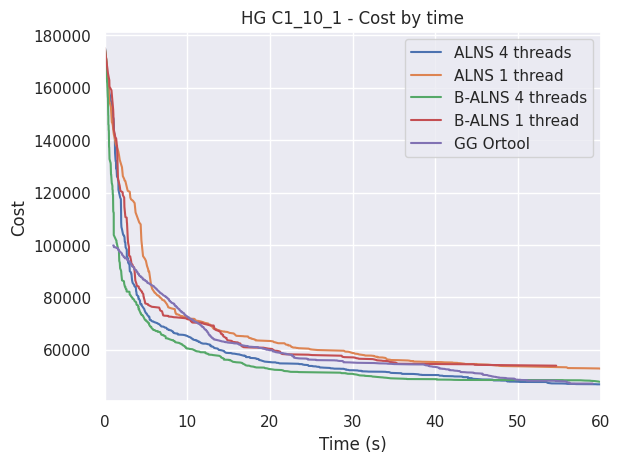
\includegraphics[width=1\linewidth]{figures/cost_time_60s_C1_10_1.png}
    \caption{60s}
    \label{fig:perf_ct_c1_10_60s}
  \end{subfigure}%
  \begin{subfigure}{.5\textwidth}
    \centering
    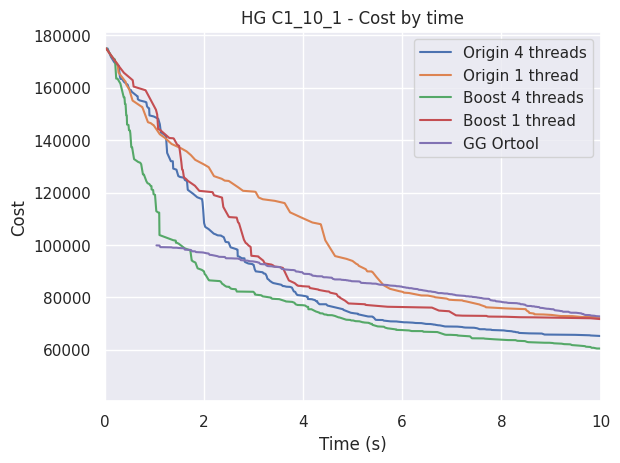
\includegraphics[width=1\linewidth]{figures/cost_time_10s_C1_10_1.png}
    \caption{10s}
    \label{fig:perf_ct_c1_10_10s}
  \end{subfigure}
  \caption{Giá trị hàm mục tiêu theo thời gian, cấu hình C1\_10\_1}
\end{figure}

\begin{figure}[H] % places figure environment here   
  \label{fig:perf_ct_r1_10}
  \begin{subfigure}{.5\textwidth}
    \centering
    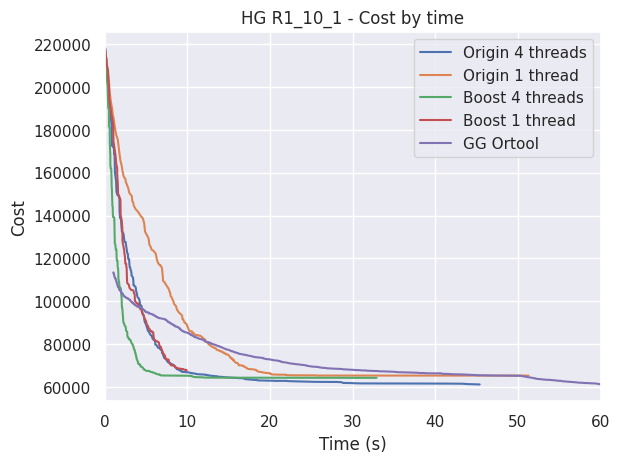
\includegraphics[width=1\linewidth]{figures/cost_time_60s_R1_10_1.png}
    \caption{60s}
    \label{fig:perf_ct_r1_10_60s}
  \end{subfigure}%
  \begin{subfigure}{.5\textwidth}
    \centering
    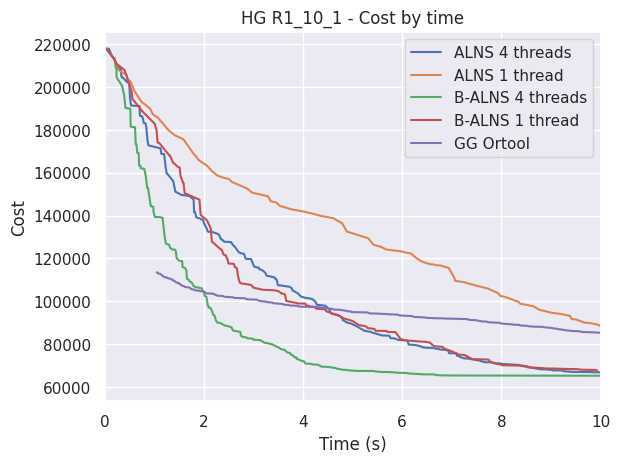
\includegraphics[width=1\linewidth]{figures/cost_time_10s_R1_10_1.png}
    \caption{10s}
    \label{fig:perf_ct_r1_10_10s}
  \end{subfigure}
  \caption{Giá trị hàm mục tiêu theo thời gian, cấu hình R1\_10\_1}
\end{figure}

\begin{figure}[H] % places figure environment here   
  \label{fig:perf_ct_rc1_10}
  \begin{subfigure}{.5\textwidth}
    \centering
    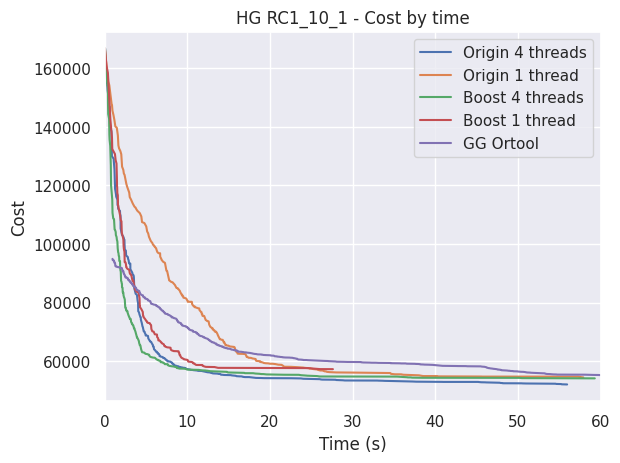
\includegraphics[width=1\linewidth]{figures/cost_time_60s_RC1_10_1.png}
    \caption{60s}
    \label{fig:perf_ct_rc1_10_60s}
  \end{subfigure}%
  \begin{subfigure}{.5\textwidth}
    \centering
    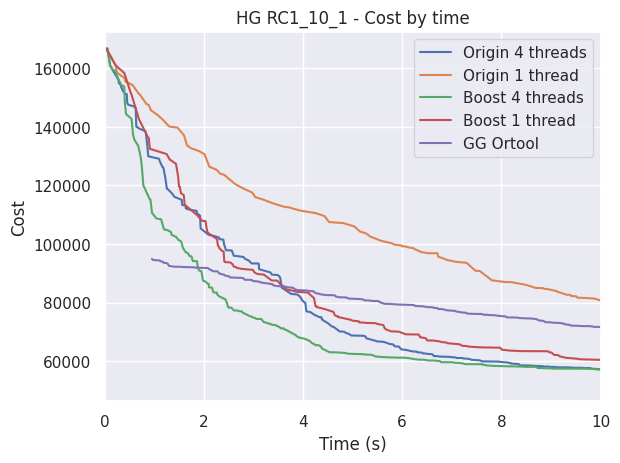
\includegraphics[width=1\linewidth]{figures/cost_time_10s_RC1_10_1.png}
    \caption{10s}
    \label{fig:perf_ct_rc1_10_10s}
  \end{subfigure}
  \caption{Giá trị hàm mục tiêu theo thời gian, cấu hình RC1\_10\_1}
\end{figure}

\begin{figure}[H] % places figure environment here   
  \label{fig:perf_ct_c1_4}
  \begin{subfigure}{.5\textwidth}
    \centering
    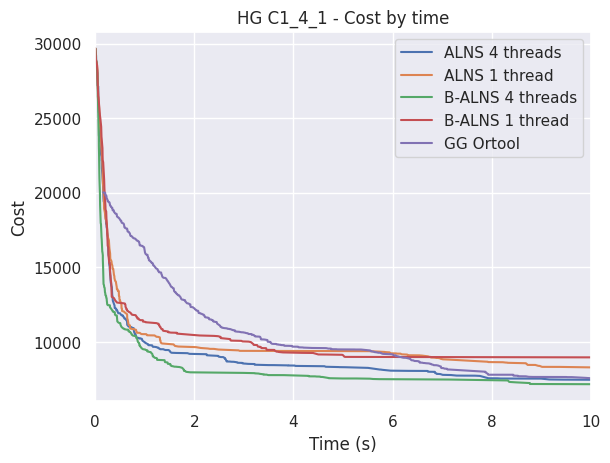
\includegraphics[width=1\linewidth]{figures/cost_time_10s_C1_4_1.png}
    \caption{10s}
    \label{fig:perf_ct_c1_4_10s}
  \end{subfigure}%
  \begin{subfigure}{.5\textwidth}
    \centering
    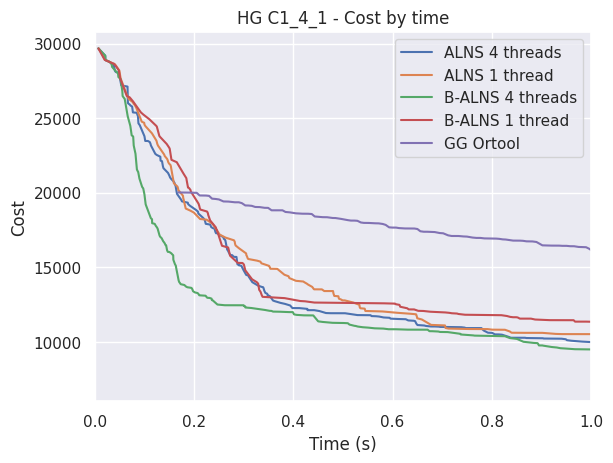
\includegraphics[width=1\linewidth]{figures/cost_time_1s_C1_4_1.png}
    \caption{1s}
    \label{fig:perf_ct_c1_4_1s}
  \end{subfigure}
  \caption{Giá trị hàm mục tiêu theo thời gian, cấu hình C1\_4\_1}
\end{figure}

\begin{figure}[H] % places figure environment here   
  \label{fig:perf_ct_r1}
  \begin{subfigure}{.5\textwidth}
    \centering
    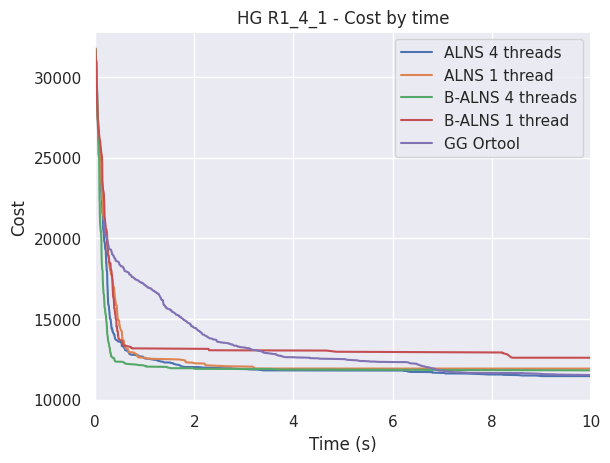
\includegraphics[width=1\linewidth]{figures/cost_time_10s_R1_4_1.png}
    \caption{10s}
    \label{fig:perf_ct_r1_60s}
  \end{subfigure}%
  \begin{subfigure}{.5\textwidth}
    \centering
    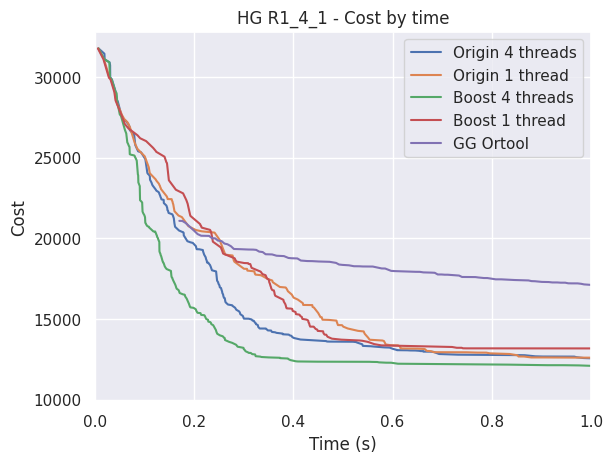
\includegraphics[width=1\linewidth]{figures/cost_time_1s_R1_4_1.png}
    \caption{1s}
    \label{fig:perf_ct_r1_10s}
  \end{subfigure}
  \caption{Giá trị hàm mục tiêu theo thời gian, cấu hình R1\_4\_1}
\end{figure}

\begin{figure}[H] % places figure environment here   
  \label{fig:perf_ct_rc1_4}
  \begin{subfigure}{.5\textwidth}
    \centering
    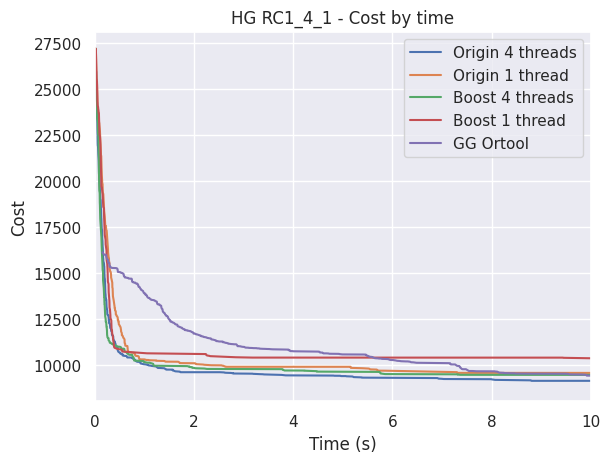
\includegraphics[width=1\linewidth]{figures/cost_time_10s_RC1_4_1.png}
    \caption{10s}
    \label{fig:perf_ct_rc1_4_10s}
  \end{subfigure}%
  \begin{subfigure}{.5\textwidth}
    \centering
    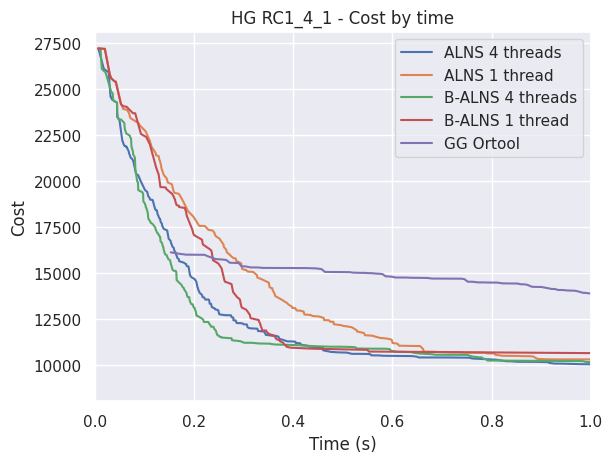
\includegraphics[width=1\linewidth]{figures/cost_time_1s_RC1_4_1.png}
    \caption{1s}
    \label{fig:perf_ct_rc1_4_1s}
  \end{subfigure}
  \caption{Giá trị hàm mục tiêu theo thời gian, cấu hình RC1\_4\_1}
\end{figure}

Với thời gian chạy lâu, các thuật toán đều chững lại bởi khi đó các tuyến đường đã khá chật chội, việc "sửa chữa" là khó khăn hơn giai đoạn đầu rất nhiều. Nói cách khác, thuật toán bị bẫy trong nghiệm tối ưu cục bộ. Khi chạy thuật toán với thời gian lâu hơn (timeout 10 phút), tác giả nhận thấy hàm mục tiêu không giảm đáng kể nữa. Chính vì thế, thời gian chạy 60 giây được lựa chọn để vừa phù hợp với thực tế và tránh việc chạy quá lâu.

Ta thấy một xu hướng rõ ràng, trong giai đoạn đầu, B-ALNS tăng tốc hiệu năng của ALNS một cách đáng kể. Với tập dữ liệu $1000$ yêu cầu, thời gian chạy dưới 10 giây, B-ALNS đơn luồng cho hiệu năng gần như tương đương với ALNS với 4 luồng. Nghĩa là, B-ALNS tiết kiệm khoảng $75\%$ tài nguyên CPU để đạt kết quả tương đương với ALNS trong thời gian chạy dưới 10 giây. Chưa kể, bộ nhớ cũng được tiết kiệm một cách đáng kể khi B-ALNS sử dụng 1 luồng thay vì 4 luồng. Khi so sánh với ALNS đơn luồng, B-ALNS đơn luồng cho hiệu năng vượt trội. Đối với tập dữ liệu có số lượng yêu cầu trung bình ($400$ yêu cầu), B-ALNS đơn luồng không có lợi thế so với ALNS đơn luồng, tuy nhiên hiệu năng đa luồng vẫn tốt hơn ALNS. Điều này cho thấy, B-ALNS có thể được sử dụng để giải quyết các bài toán lớn với tài nguyên hạn chế. Với cấu hình $400$ yêu cầu, B-ALNS đa luồng cho hiệu năng bỏ xa ALNS với thời gian chạy dưới $0.2$ giây và luôn tốt hơn trong thời gian chạy dưới $1$ giây.

Khi so sánh với \code{Google OR-Tools}, ta thấy rằng, \code{Google OR-Tools} cho hiệu năng tốt trong thời gian chạy từ 2 đến 4 giây đầy tiên (tập $1000$ yêu cầu). Tuy nhiên với thời gian chạy dưới 1 giây, \code{Google OR-Tools} không thể cho ra kết quả. Với thời gian chạy lâu hơn, \code{Google OR-Tools} cho hiệu năng không tốt bằng ALNS hay B-ALNS. Với cấu hình $400$ yêu cầu, nhìn chung hiệu năng của B-ALNS cũng như ALNS bỏ xa \code{Google OR-Tools}.

Như vậy đối với các nghiệp vụ yêu cầu một kết quả tốt trong thời gian ngắn, B-ALNS là lựa chọn tốt nhất. Khi tiến hành đo đạc với thời gian chạy dài (timeout lớn hơn 1 phút), tác giả nhận thấy rằng, ALNS là tốt nhất trong các thuật toán được đề cập ở đây. Tuy nhiên chất lượng nghiệm tốt hơn B-ALNS thường không quá $1\%$. Các kết quả được chỉ ra trong phần trước là giá trị hàm mục tiêu khi sử dụng ALNS nguyên bản.

\subsection{Số xe}

Chúng ta cũng nhận thấy một xu hướng tương tự như khi so sánh hiệu năng của các thuật toán khi sử dụng độ đo là giá trị hàm mục tiêu. B-ALNS cho hiệu năng vượt trội trong giai đoạn đầu. B-ALNS đơn luồng cho hiệu năng tương đương với ALNS với 4 luồng. Với cấu hình lớp R ($1000$ yêu cầu), B-ALNS tiết kiệm được khoảng $30\%$ số xe so với ALNS trong thời gian chạy từ 2 tới 4 giây! Tương tự, với cấu hình $400$ yêu cầu, B-ALNS giảm số xe nhanh hơn đáng kể so với ALNS trong thời gian chạy ngắn (dưới $0.2$ giây).  Việc tiết kiệm hàng trăm xe có ý nghĩa rất lớn trong thực tế. Thường thì chi phí cho một xe (thuê, hoặc mua, nhiên liệu, chi phí cho tài xế, ...) là rất lớn. Việc tiết kiệm số xe sẽ giúp giảm chi phí vận hành của doanh nghiệp một cách đáng kể. 

Với thời gian chạy lâu hơn, đương nhiên chúng ta rất khó để giảm được số xe nữa, vì hầu hết các tuyến đường đến lúc này đã chật chội hơn đáng kể so với giai đoạn đầu.

\begin{figure}[H] % places figure environment here   
  \label{fig:perf_ct_c1_10}
  \begin{subfigure}{.5\textwidth}
    \centering
    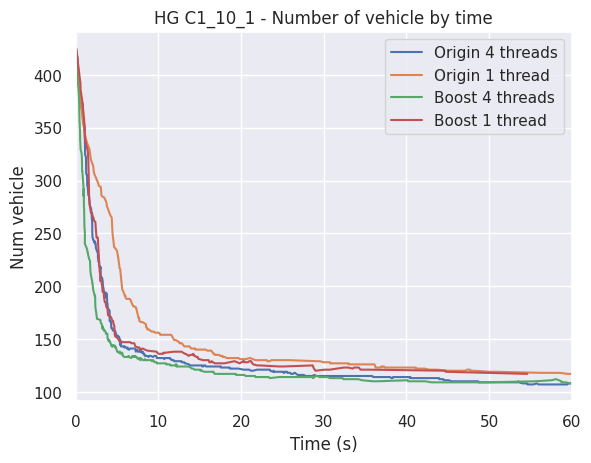
\includegraphics[width=0.9\linewidth]{figures/nv_time_60s_C1_10_1.png}
    \caption{60s}
    \label{fig:perf_ct_c1_10_60s}
  \end{subfigure}%
  \begin{subfigure}{.5\textwidth}
    \centering
    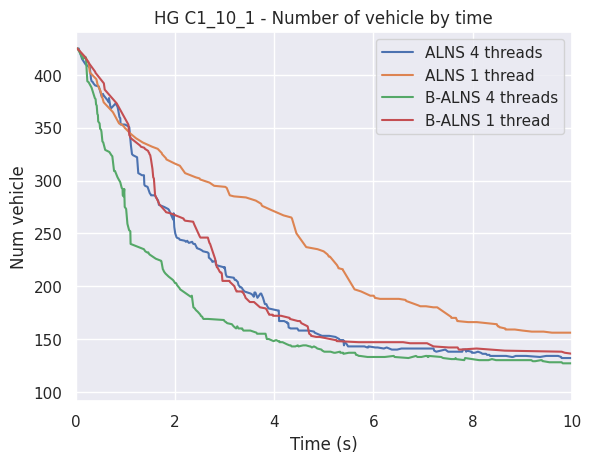
\includegraphics[width=0.9\linewidth]{figures/nv_time_10s_C1_10_1.png}
    \caption{10s}
    \label{fig:perf_ct_c1_10_10s}
  \end{subfigure}
  \caption{Số xe sử dụng theo thời gian, cấu hình C1\_10\_1}
\end{figure}

\begin{figure}[H] % places figure environment here   
  \label{fig:perf_ct_r1_10}
  \begin{subfigure}{.5\textwidth}
    \centering
    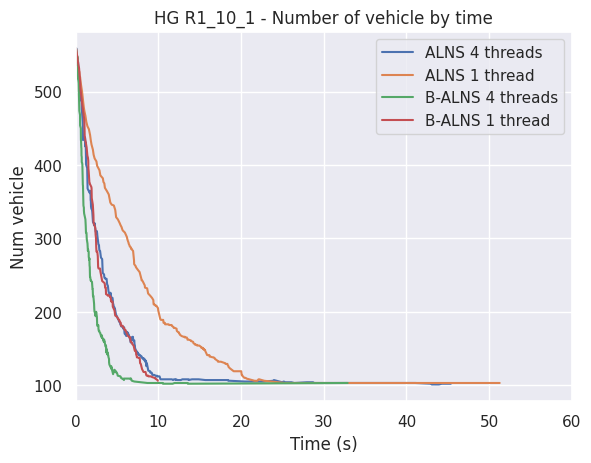
\includegraphics[width=0.9\linewidth]{figures/nv_time_60s_R1_10_1.png}
    \caption{60s}
    \label{fig:perf_ct_r1_10_60s}
  \end{subfigure}%
  \begin{subfigure}{.5\textwidth}
    \centering
    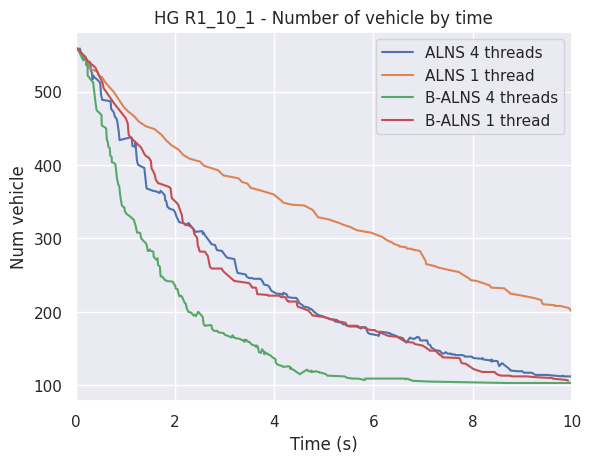
\includegraphics[width=0.9\linewidth]{figures/nv_time_10s_R1_10_1.png}
    \caption{10s}
    \label{fig:perf_ct_r1_10_10s}
  \end{subfigure}
  \caption{Số xe sử dụng theo thời gian, cấu hình R1\_10\_1}
\end{figure}

\begin{figure}[H] % places figure environment here   
  \label{fig:perf_ct_rc1}
  \begin{subfigure}{.5\textwidth}
    \centering
    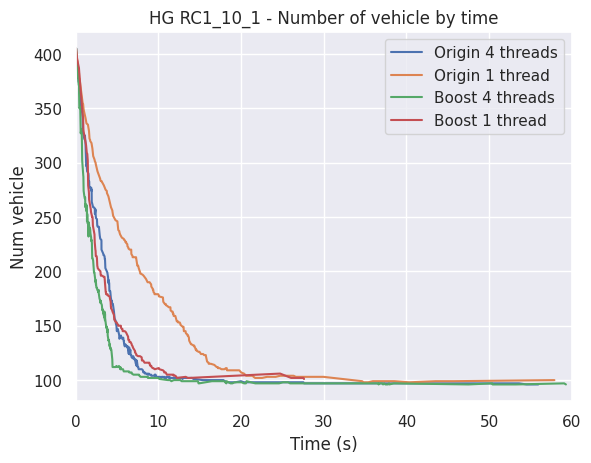
\includegraphics[width=0.9\linewidth]{figures/nv_time_60s_RC1_10_1.png}
    \caption{60s}
    \label{fig:perf_ct_rc1_60s}
  \end{subfigure}%
  \begin{subfigure}{.5\textwidth}
    \centering
    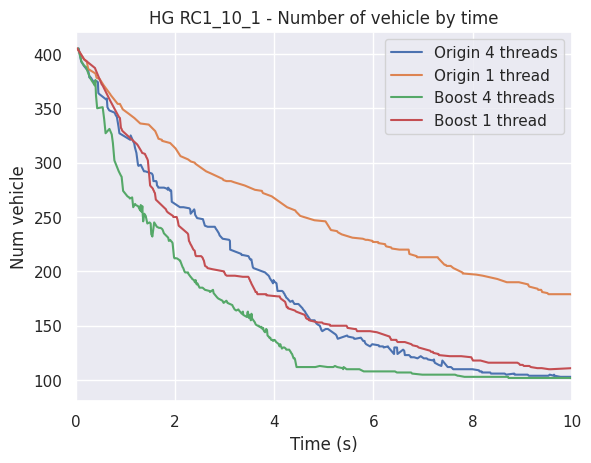
\includegraphics[width=0.9\linewidth]{figures/nv_time_10s_RC1_10_1.png}
    \caption{10s}
    \label{fig:perf_ct_rc1_10s}
  \end{subfigure}
  \caption{Số xe sử dụng theo thời gian, cấu hình RC1\_10\_1}
\end{figure}

\begin{figure}[H] % places figure environment here   
  \label{fig:perf_ct_c1_4}
  \begin{subfigure}{.5\textwidth}
    \centering
    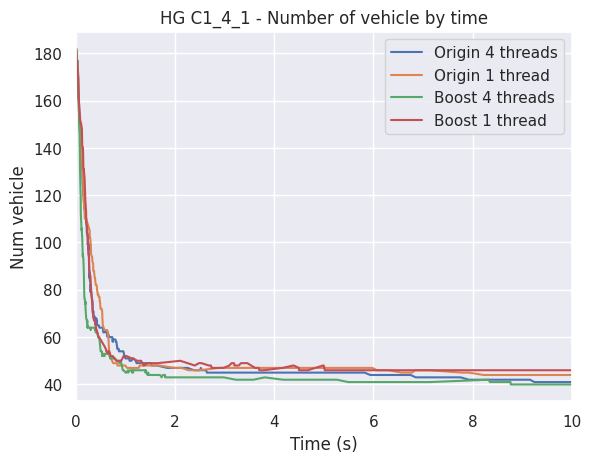
\includegraphics[width=0.9\linewidth]{figures/nv_time_10s_C1_4_1.png}
    \caption{10s}
    \label{fig:perf_ct_c1_4_10s}
  \end{subfigure}%
  \begin{subfigure}{.5\textwidth}
    \centering
    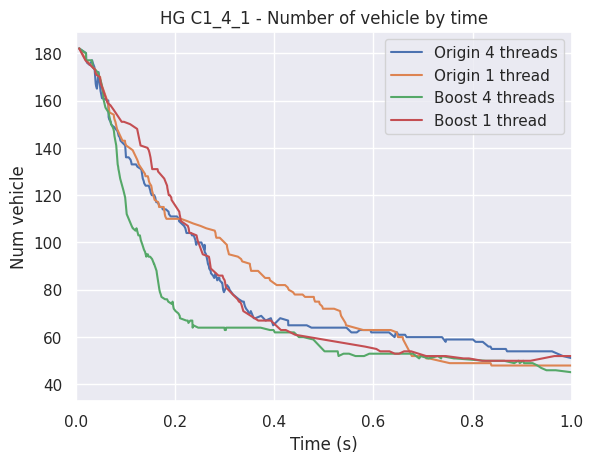
\includegraphics[width=0.9\linewidth]{figures/nv_time_1s_C1_4_1.png}
    \caption{1s}
    \label{fig:perf_ct_c1_4_1s}
  \end{subfigure}
  \caption{Số xe sử dụng theo thời gian, cấu hình C1\_4\_1}
\end{figure}

\begin{figure}[H] % places figure environment here   
  \label{fig:perf_ct_r1_4}
  \begin{subfigure}{.5\textwidth}
    \centering
    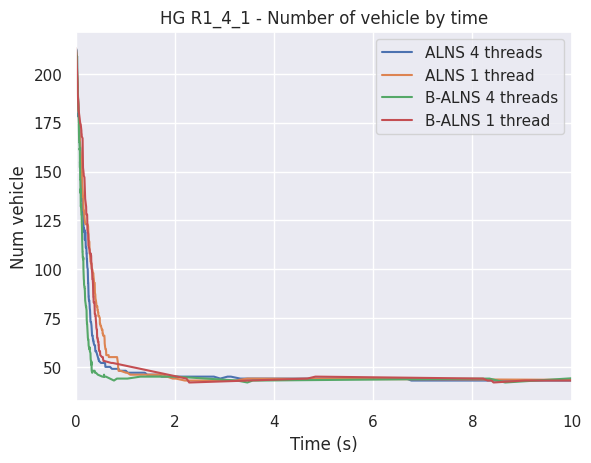
\includegraphics[width=0.9\linewidth]{figures/nv_time_10s_R1_4_1.png}
    \caption{10s}
    \label{fig:perf_ct_r1_4_10s}
  \end{subfigure}%
  \begin{subfigure}{.5\textwidth}
    \centering
    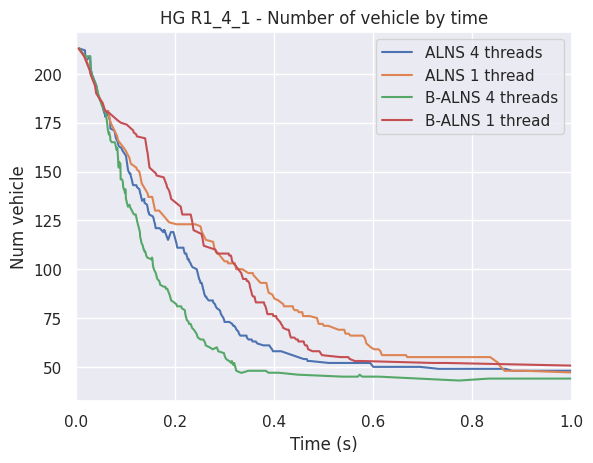
\includegraphics[width=0.9\linewidth]{figures/nv_time_1s_R1_4_1.png}
    \caption{1s}
    \label{fig:perf_ct_r1_4_1s}
  \end{subfigure}
  \caption{Số xe sử dụng theo thời gian, cấu hình R1\_4\_1}
\end{figure}

\begin{figure}[H] % places figure environment here   
  \label{fig:perf_ct_rc1}
  \begin{subfigure}{.5\textwidth}
    \centering
    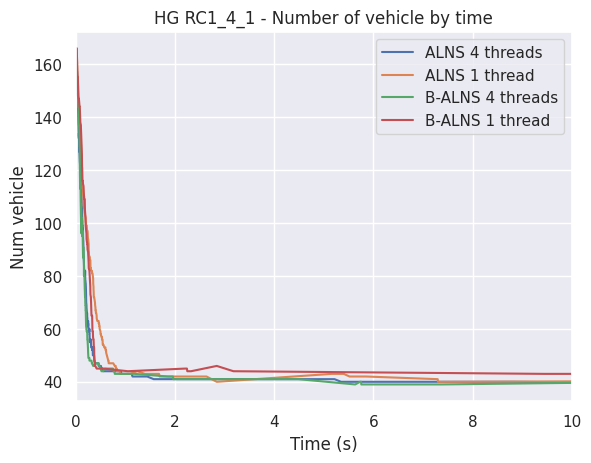
\includegraphics[width=0.9\linewidth]{figures/nv_time_10s_RC1_4_1.png}
    \caption{10s}
    \label{fig:perf_ct_rc1_4_10s}
  \end{subfigure}%
  \begin{subfigure}{.5\textwidth}
    \centering
    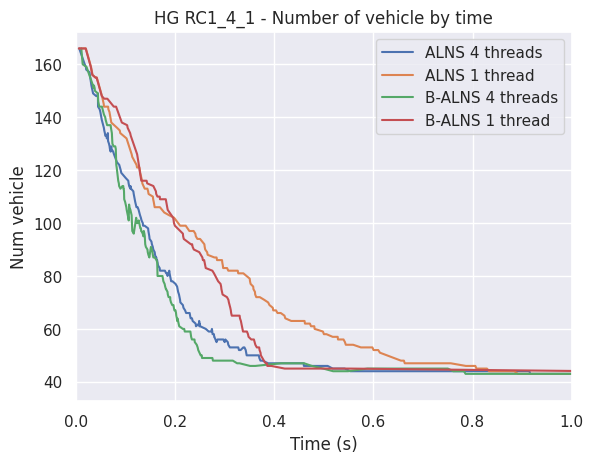
\includegraphics[width=0.9\linewidth]{figures/nv_time_1s_RC1_4_1.png}
    \caption{1s}
    \label{fig:perf_ct_rc1_4_1s}
  \end{subfigure}
  \caption{Số xe sử dụng theo thời gian, cấu hình RC1\_4\_1}
\end{figure}
\section{Tần suất sử dụng thuật toán hủy, chèn}

Trong phần này, chúng ta sẽ theo dõi trọng số của các thuật toán hủy, chèn qua các vòng lặp. Từ đó ta biết được rằng liệu thuật toán hủy hay chèn có hiệu quả (trọng số cao) hay không hay các thuật toán hủy, chèn đó hiệu quả (hoặc không) vào giai đoạn nào của ALNS.
 
\begin{figure}[H] % places figure environment here   
	\centering % Centers Graphic
	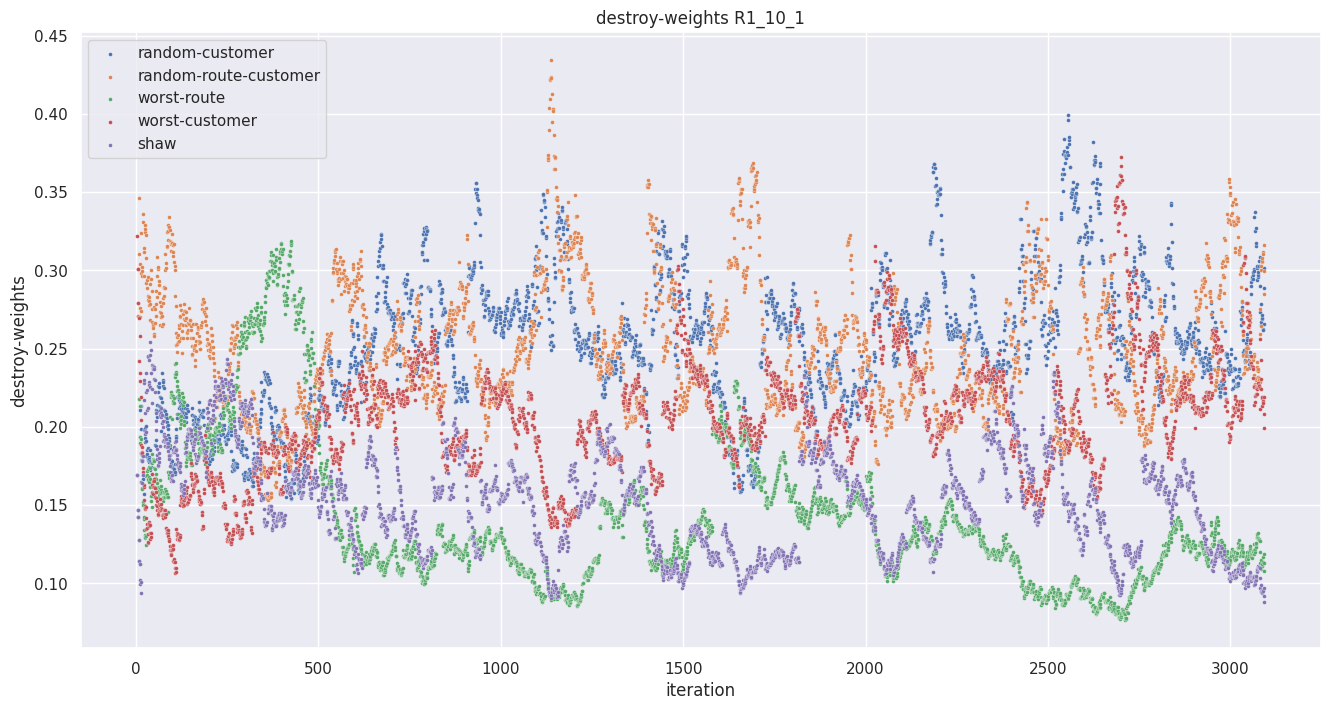
\includegraphics[width=1\textwidth]{figures/destroy_weights_R1_10_1.png}
	% \includesvg[scale=1]{figures/core-object}
	\caption{Trọng số của các thuật toán hủy}
	\label{fig:alg_01}
\end{figure}

\begin{figure}[H] % places figure environment here   
	\centering % Centers Graphic
	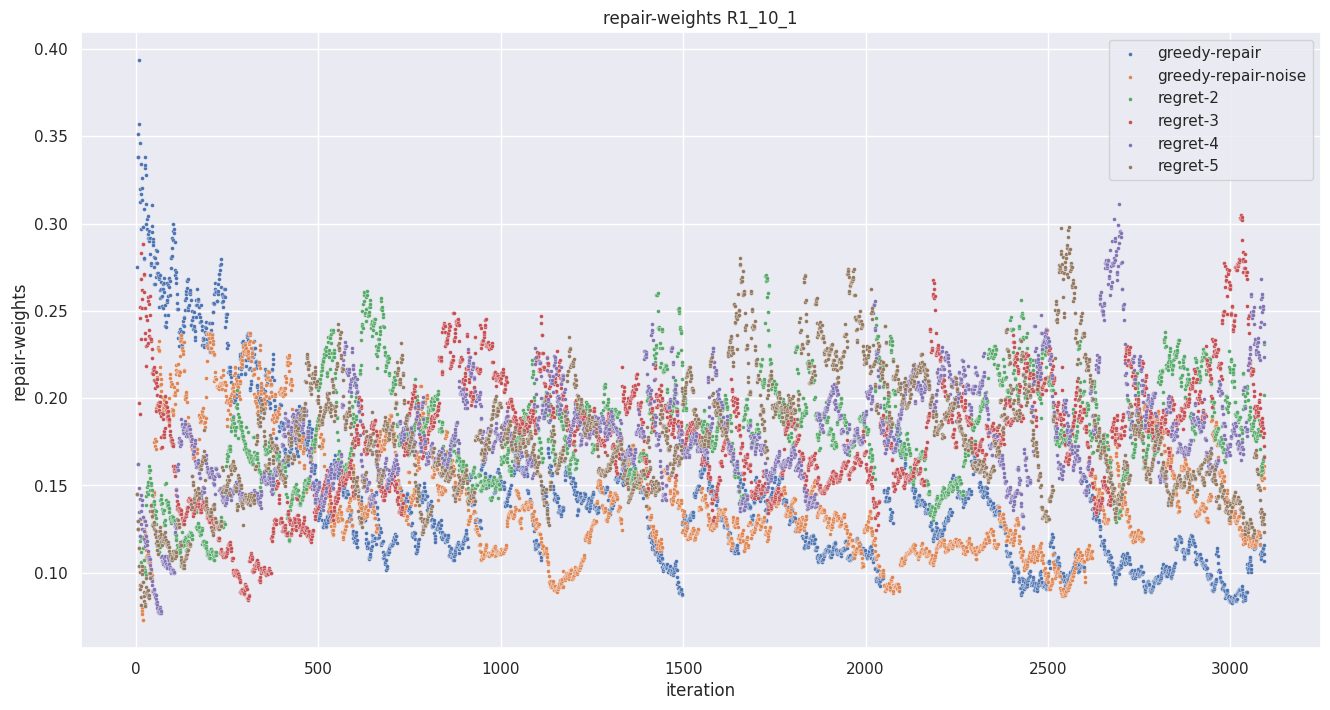
\includegraphics[width=1\textwidth]{figures/repair_weights_R1_10_1.png}
	% \includesvg[scale=1]{figures/core-object}
	\caption{Trọng số của các thuật toán chèn}
	\label{fig:alg_02}
\end{figure}

\subsection*{Thuật toán hủy}
Trong giai đoạn đầu của ALNS, thuật toán \textit{hủy tuyến tệ} được sử dụng nhiều (trọng số cao) nhưng về sau thì tần suất sử dụng lại giảm dần. Không khó hiểu khi ban đầu, các tuyến được sắp xếp chưa thực sự hiệu quả nên ta có thể xóa toàn bộ yêu cầu trong một số tuyến nhất định và chèn vào các tuyến khác. Đến giai đoạn sau của ALNS, khi các tuyến đường đã chứa những yêu cầu quan trọng (nghĩa là rất khó để chèn chúng vào một tuyến đường khác), ta khó có thể xóa cả tuyến đường. Việc thuật toán hủy tuyến được sử dụng nhiều vào giai đoạn đầu của ALNS giúp giảm nhanh số xe được sử dụng. Thực chất, ta cũng chỉ muốn sử dụng hủy tuyến vào giai đoạn đầu của thuật toán. ALNS tự điều chỉnh trọng số của các thuật toán hủy, chèn khiến chúng ta không cần phải thiết lập phức tạp trong khi cài đặt, ví dụ như ta chỉ muốn thuật toán hủy, chèn nhất định được sử dụng trong giai đoạn nào đó trong quá trình chạy ALNS. 

Ngược lại với thuật toán \textit{hủy tuyến tệ}, thuật toán \textit{hủy yêu cầu tệ} cho thấy hiệu quả vào giai đoạn sau của ALNS. Thuật toán \textit{hủy yêu cầu ngẫu nhiên}, \textit{hủy yêu cầu ngẫu nhiên với tuyến} hay thuật toán hủy \textit{Shaw} cho thấy sự "ổn định" khi luôn giữ trọng số cao trong suốt quá trình chạy ALNS.

\subsection*{Thuật toán chèn}
Đối với các thuật toán chèn, ta thấy rõ sự hiệu quả của nhóm các thuật toán \textit{hối tiếc} khi so sánh với nhóm \textit{tham lam} khi trong suốt quá trình chạy, các thuật toán chèn \textit{hối tiếc} luôn giữ trọng số cao. Trong giai đoạn đầu, nhóm thuật toán chèn tham lam giữ trọng số cao, tuy nhiên sau đó, chúng có xu hướng giảm và tỏ ra không còn hiệu quả như nhóm các thuật toán \textit{hối tiếc}.
\section{Kĩ thuật tăng nhiệt}
\label{sec:reheat}
Một trong những vấn đề mà nhiều thuật toán tìm kiếm lân cận gặp phải đó là bị mắc trong một nghiệm tối ưu địa phương. Điều này có nghĩa là, sau một khoảng thời gian tìm kiếm ta thấy rằng thuật toán không thể cải thiện nghiệm thêm nữa hoặc là qua rất nhiều bước lặp nữa mới tìm được một nghiệm tốt hơn. Có nhiều yếu tố ảnh hưởng đến hiện tượng này. Ví dụ, đối với ALNS, số lượng yêu cầu bỏ đi quá lớn hoặc quá nhỏ khiến cho các thuật toán chèn không tìm được vị trí tốt để thêm lại yêu cầu (khi mà các tuyến đã chật chội sau một khoảng thời gian chạy). Ngoài ra, tiêu chí chấp nhận nghiệm cũng ảnh hưởng rất nhiều. Đối với mô phỏng luyện kim, càng về sau chúng ta chỉ chấp nhận những nghiệm tốt hơn nghiệm tốt nhất đã biết hoặc là chấp nhận một nghiệm tệ hơn với giá trị chênh lệch rất nhỏ do tham số "nhiệt độ" của mô phỏng luyện kim đã nhỏ đi đáng kể sau thời gian chạy dài. Để khắc phục hiện tượng này, ta có thể sử dụng kĩ thuật tăng nhiệt (\textit{reheat}) để tăng "nhiệt độ" của mô phỏng luyện kim lên một giá trị nào đó trong những giai đoạn nhất định (Salwani và các cộng sự (2011) \cite{salwani2011re}). 

Có một vài cách tăng nhiệt khác nhau ví dụ như tăng nhiệt khi sau một số vòng lặp mà thuật toán không cải thiện được nghiệm hoặc tăng nhiệt sau một số vòng lặp nhất định (cố định). Trong quá trình thực nghiệm cho luận văn này, cách thứ hai được sử dụng. Tăng nhiệt không cần thiết phải sử dụng với các cấu hình quá nhỏ hoặc thời gian chạy ngắn vì nó cũng không tìm ra nghiệm tốt hơn (đáng kể) khi không sử dụng. 

Nhiệt độ mới được cho bởi công thức
\begin{equation}
  T_{new} = T_{old} \times \alpha,
\end{equation}
trong đó, $T_{old}$ là nhiệt độ tại lần cuối cùng thuật toán tìm được nghiệm mới cải thiện so với nghiệm hiện tại, $T_{new}$ là nhiệt độ mới và $\alpha$ là hệ số tăng nhiệt được cấu hình từ đầu.

\begin{figure}[H] % places figure environment here   
  \centering % Centers Graphic
  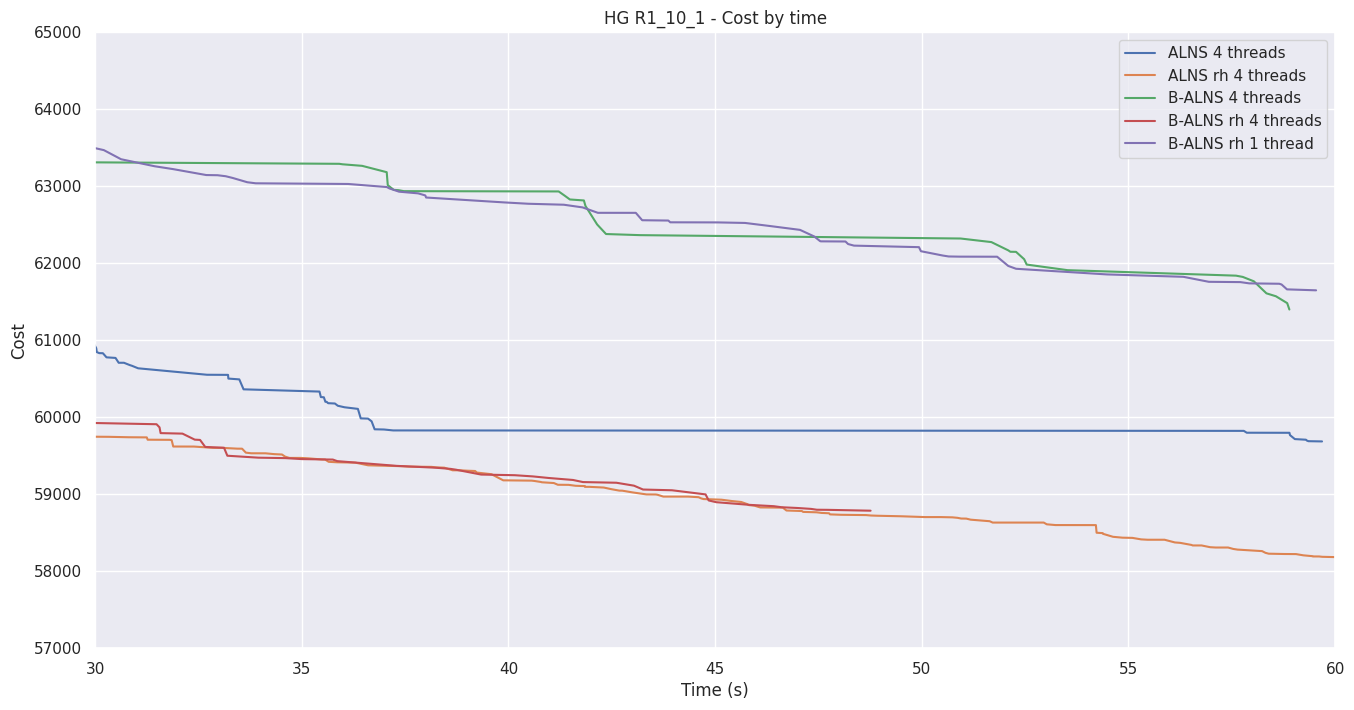
\includegraphics[width=1\textwidth]{figures/cost_time_R1_10_1_rh.png} 
  % \includesvg[scale=1]{figures/core-object}
  \caption{Hàm mục tiêu theo thời gian với một số cách chạy khác nhau cho cấu hình \code{R1\_10\_1} (\textit{rh biểu thị cho các thuật toán áp dụng kĩ thuật tăng nhiệt}).} 
  \label{fig:reheat1}
\end{figure}

Một điểm thú vị là kĩ thuật tăng nhiệt giúp cho B-ALNS "thoát" được nghiệm tối ưu địa phương khi đã trải qua thời gian chạy dài. Không những vậy tăng nhiệt giúp các thuật toán tìm được nghiệm tốt hơn khi so với không dùng tăng nhiệt.